\documentclass[pdf]{beamer}
%\mode<presentation>{}

\usepackage{amssymb,amsmath,amsthm,enumerate,mathtools}
\usepackage[utf8]{inputenc}
\usepackage{array}
\newcolumntype{C}[1]{>{\centering\arraybackslash}m{#1}}

\usepackage[parfill]{parskip}
\usepackage{graphicx}
\usepackage{caption}
\captionsetup[figure]{labelformat=empty}
\usepackage{subcaption}
\usepackage{bm}
\usepackage{amsfonts,amscd}
%\usepackage{gensymb}
\usepackage[]{units}
\usepackage{listings}
\usepackage{multicol}
\usepackage{tcolorbox}
\usepackage{physics}
\usepackage{multirow}
\usepackage{pgfplots,tikz}
\pgfplotsset{compat=1.7}
\usepackage{hyperref}
\hypersetup{
    colorlinks=true,
    linkcolor=franklinblue,
    filecolor=magenta,      
    urlcolor=cyan,
    bookmarks=true,
    citecolor= black
    % pdftitle={Overleaf Example},
    % pdfpagemode=FullScreen,
    }
\usepackage{colortbl}
\usepackage{booktabs}
\usepackage{gensymb}
\usepackage{color}
\usepackage{natbib}

\usepackage{tikz}
\usepackage{fixltx2e}
\usepackage[english]{babel}
\usepackage[absolute,overlay]{textpos}
%\usepackage{gnuplottex} % For t-distribution using gnuplot.
%The following function is use in students t distribution. 
% \def\basefunc{    gamma((\n+1)/2.)/(sqrt(\n*pi)*gamma(\n/2.))*((1+(x*x)/\n)^(-(\n+1)/2.))}    
% \def\n{7}
%\usepackage{tkz-fct} % For t-distribution plotting.
% \usepackage{pst-func} % For t-distribution plotting.
\usepackage{longtable}
\usepackage{changepage} 

\usetikzlibrary{shapes,decorations,arrows,calc,arrows.meta,fit,positioning}
\tikzset{
    -Latex,auto,node distance =1 cm and 1 cm,semithick,
    state/.style ={ellipse, draw, minimum width = 0.7 cm},
    point/.style = {circle, draw, inner sep=0.04cm,fill,node contents={}},
    bidirected/.style={Latex-Latex,dashed},
    el/.style = {inner sep=2pt, align=left, sloped}
}

%Normal Distribution
\pgfmathdeclarefunction{gauss_}{2}{\pgfmathparse{1/(#2*sqrt(2*pi))*exp(-((x-#1)^2)/(2*#2^2))}%
}
%Gamma Distribution
\pgfmathdeclarefunction{gammaPDF}{2}{
\pgfmathparse{1/(#2^#1*gamma(#1))*x^(#1-1)*exp(-x/#2)}
}

%%%%% For https://tikz.net/gaussians/ %%%%%

\usepackage{amsmath} % for \dfrac
\usepackage{tikz}
\tikzset{>=latex} % for LaTeX arrow head
\usepackage{pgfplots} % for the axis environment
\usepackage{xcolor}
\usepackage[outline]{contour} % halo around text
\contourlength{1.2pt}
\usetikzlibrary{positioning,calc}
\usetikzlibrary{backgrounds}% required for 'inner frame sep'
%\usepackage{adjustbox} % add whitespace (trim)

% define gaussian pdf and cdf
\pgfmathdeclarefunction{gauss}{3}{%
  \pgfmathparse{1/(#3*sqrt(2*pi))*exp(-((#1-#2)^2)/(2*#3^2))}%
}
\pgfmathdeclarefunction{cdf}{3}{%
  \pgfmathparse{1/(1+exp(-0.07056*((#1-#2)/#3)^3 - 1.5976*(#1-#2)/#3))}%
}
\pgfmathdeclarefunction{fq}{3}{%
  \pgfmathparse{1/(sqrt(2*pi*#1))*exp(-(sqrt(#1)-#2/#3)^2/2)}%
}
\pgfmathdeclarefunction{fq0}{1}{%
  \pgfmathparse{1/(sqrt(2*pi*#1))*exp(-#1/2))}%
}

\colorlet{mydarkblue}{blue!30!black}

% to fill an area under function
\usepgfplotslibrary{fillbetween}
\usetikzlibrary{patterns}
\pgfplotsset{compat=1.12} % TikZ coordinates <-> axes coordinates
% https://tex.stackexchange.com/questions/240642/add-vertical-line-of-equation-x-2-and-shade-a-region-in-graph-by-pgfplots

% plot aspect ratio
%\def\axisdefaultwidth{8cm}
%\def\axisdefaultheight{6cm}

% number of sample points
\def\N{50}

%%%%% End for https://tikz.net/gaussians/ %%%%%

\setbeamertemplate{caption}[numbered]

%new commands
\newcommand{\der}[2]{\frac{d#1}{d#2}}
\newcommand{\nder}[3]{\frac{d^#1 #2}{d #3 ^ #1}}
\newcommand{\pder}[2]{\frac{\partial #1}{\partial #2}}
\newcommand{\npder}[3]{\frac{\partial ^#1 #2}{\partial #3^#1}}
\newcommand{\sentencelist}{def}
\newcommand{\overbar}[1]{\mkern 1.5mu\overline{\mkern-1.5mu#1\mkern-1.5mu}\mkern 1.5mu}
\newcommand{\lined}{\overbar}
\newcommand{\perm}[2]{{}^{#1}\!P_{#2}}
\newcommand{\comb}[2]{{}^{#1}C_{#2}}
\newcommand{\intall}{\int_{-\infty}^{\infty}}
\newcommand{\Var}[1]{\text{Var}\left(#1\right)}
\newcommand{\E}[1]{\text{E}\left(#1\right)}
\newcommand{\define}{\equiv}
\newcommand{\diff}[1]{\mathrm{d}#1}
\newcommand{\empy}[1]{{\color{cadetblue}\texttt{#1}}}
\newcommand{\empr}[1]{{\color{franklinblue}\textbf{#1}}}
%https://tex.stackexchange.com/questions/192358/quickly-changing-all-the-file-paths-in-a-tex-file
%\newcommand{\pathtopdf}{C:/Users/bkwei/OneDrive - Franklin University/Desktop/Math_215/Data/IMDB/Processed} - Not Tested!
\newcolumntype{L}[1]{>{\raggedright\let\newline\\\arraybackslash\hspace{0pt}}m{#1}}
\newcolumntype{C}[1]{>{\centering\let\newline\\\arraybackslash\hspace{0pt}}m{#1}}
\newcolumntype{R}[1]{>{\raggedleft\let\newline\\\arraybackslash\hspace{0pt}}m{#1}}

\theoremstyle{remark}
\newtheorem*{remark}{Remark}
\theoremstyle{definition}

\newcommand{\examplebox}[2]{
\begin{tcolorbox}[colframe=darkcardinal,colback=boxgray,title=#1]
\end{tcolorbox}}

\newcommand{\eld}[1]{\frac{d}{dt}(\frac{\partial L}{\partial \dot #1}) - \frac{\partial L}{\partial #1}=0}
\newcommand{\euler}[1]{\frac{\partial L}{\partial #1}-\frac{d}{dt}(\frac{\partial L}{\partial \dot #1})}
\newcommand{\eulerg}[1]{\frac{\partial g}{\partial #1}-\frac{d}{dt}(\frac{\partial g}{\partial \dot #1})}
\newcommand{\divg}[1]{\nabla\cdot #1}
\newcommand{\prob}[1]{P(#1\vert I)}

\AtBeginSection[]{
  \begin{frame}
  \vfill
  \centering
  \begin{beamercolorbox}[sep=8pt,center,%shadow=true,
  rounded=true]{section}
    \LARGE
    \usebeamerfont{section}
    %\usebeamercolor[fg]{section}\inserttitle %\insertsectionhead\par%
    \setbeamercolor{section}{fg=white,bg=white}\insertsectionhead\par%
  \end{beamercolorbox}
  \vfill
  \end{frame}
}

\usetheme{Franklin} 
\def \i  {\item}
\def \ai {\item[] \quad \arrowbullet}
\newcommand \si[1]{\item[] \quad \bulletcolor{#1}}
\def \wi {\item[] \quad $\ \phantom{\Rightarrow}\ $}
\def \bi {\begin{itemize}\item}
\def \ei {\end{itemize}}
\def \be {\begin{equation*}}
\def \ee {\end{equation*}}
\def \bie {$\displaystyle{}
\def \eie {{\ }$}}
\def \bsie {\small$\displaystyle{}
\def \esie {{\ }$}\normalsize\selectfont}
\def \bse {\small\begin{equation*}}
\def \ese {\end{equation*}\normalsize}
\def \bfe {\footnotesize\begin{equation*}}
\def \efe {\end{equation*}\normalsize}
\renewcommand \le[1] {\\ \medskip \lefteqn{\hspace{1cm}#1} \medskip}
\def \bex {\begin{example}}
\def \eex {\end{example}}
\def \bfig {\begin{figure}}
\def \efig {\end{figure}}
\def \btheo {\begin{theorem}}
\def \etheo {\end{theorem}}
\def \bc {\begin{columns}}
\def \ec {\end{columns}}
\def \btab {\begin{tabbing}}
\def \etab {\end{tabbing}\svneg\svneg}
\newcommand \col[1]{\column{#1\linewidth}}
\def\vneg  {\vspace{-5mm}}
\def\lvneg {\vspace{-10mm}}
\def\svneg {\vspace{-2mm}}
\def\tvneg {\vspace{-1mm}}
\def\vpos  {\vspace{5mm}}
\def\lvpos {\vspace{10mm}}
\def\svpos {\vspace{2mm}}
\def\tvpos {\vspace{1mm}}
\def\hneg  {\hspace{-5mm}}
\def\lhneg {\hspace{-10mm}}
\def\shneg {\hspace{-2mm}}
\def\thneg {\hspace{-1mm}}
\def\hpos  {\hspace{5mm}}
\def\lhpos {\hspace{10mm}}
\def\shpos {\hspace{2mm}}

\logo{
\includegraphics[height=0.4in]{./style_files_franklin/FranklinUniversity_TM1.jpg}}

\title{BUSA 603}
\subtitle{Module 2:   Marketing Analytics Tools \& Data Platforms}

\beamertemplatenavigationsymbolsempty

\begin{document}

\author[B. Weikel, Franklin University]{
	\begin{tabular}{c} 
	\Large
	Brian Weikel\\
    \footnotesize \href{mailto:brian.weikel@franklin.edu}{brian.weikel@franklin.edu}
    \vspace{1ex}
\end{tabular}
\vspace{-4ex}}

\institute{
	
\includegraphics[height=0.4in]{./style_files_franklin/FranklinUniversity_TM1.jpg}\\
	Business Analytics\\
	Franklin University}

\date{Spring 2024}%{\today}

\begin{noheadline}
\begin{frame}[t]\maketitle\end{frame}
\end{noheadline}

\begin{frame}[t]{Outline\footnote{These lecture notes map to chapters 2 and 5 of \cite{davis2022}.}}
\begin{enumerate}
\item Spreadsheet Tools 
\vspace{1.0ex}
\item Programming Tools
\vspace{1.0ex}
\item Variables and Variable Types
\vspace{1.0ex}
\item First, Second and Third Party Data
\vspace{1.0ex}
\item Data Management Platforms
\vspace{1.0ex}
\item Marketing Measurement and Optimization Solutions
\vspace{1.0ex}
\item Data Collection Laws
\vspace{1.0ex}
\item Appendix
\end{enumerate}
\end{frame}

\section{Spreadsheet Tools}

\begin{frame}[t]{Excel}
A \empr{spreadsheet tool} is an interactive software application for structuring, transforming, analyzing and storing data in rows and columns.  You will hear people say such data is in a \textit{tabular format}.
 \\
 \vspace{1.5ex}
\empr{Tabular format}, or  \empr{tabular form}, is simply information presented in the form of a table with rows and columns. \\
\vspace{1.5ex}
With the proper permissions and syntax, \href{https://www.microsoft.com/en-us/microsoft-365/excel}{Excel} has the capabilities to read data from a host of sources or platforms. \\
\vspace{1.5ex}
Via the Excel ribbon, choose \texttt{Draw} and then \texttt{Get Data} to review potential sources and platforms.  
\end{frame}

\begin{frame}[t]{Excel \texttt{Data} $\rightarrow$ \texttt{Get Data} $\rightarrow$ \texttt{From File} Options}
\begin{figure}[htbp]
  \captionsetup{justification=centering}
  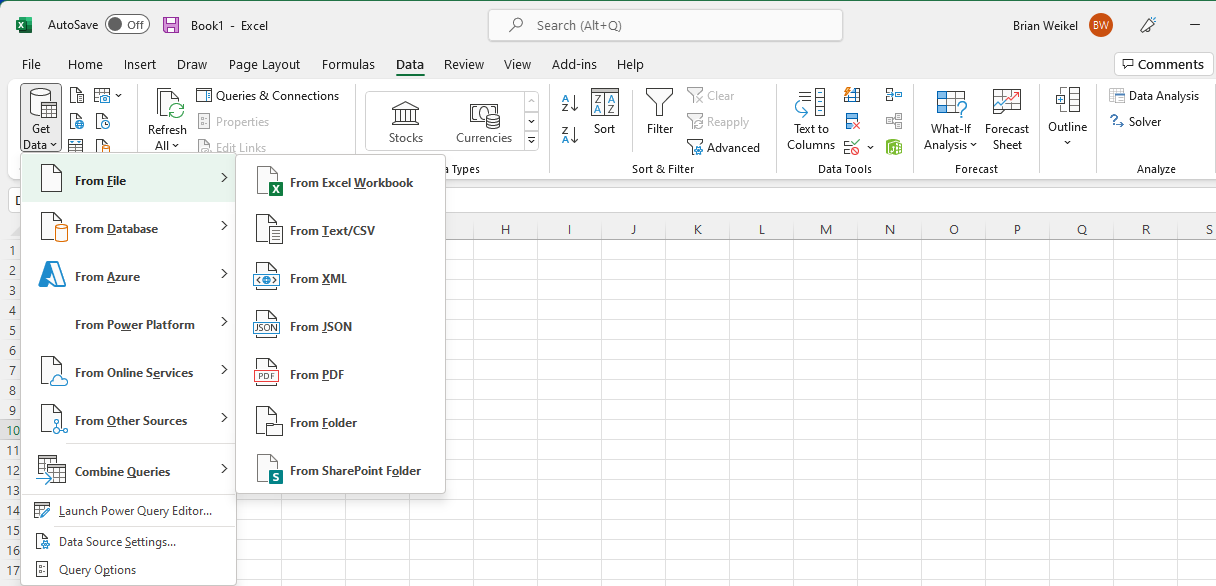
\includegraphics[height=2in, trim=0.0cm 0.0cm 0.0cm 0.0cm width=6in]{Images/Excel_1.png}
  \caption{Figure {\color{franklinblue} 1}: Excel \texttt{From File} Options}
\end{figure}
\vspace{-1.5ex}
Options frequently used to read data into Excel include \texttt{Excel Workbooks}, \texttt{Text/CSV} files, and \texttt{JSON}.
\end{frame}


\begin{frame}[t]{Excel \texttt{Data} $\rightarrow$ \texttt{Get Data} $\rightarrow$ \texttt{From Database} Options}
\begin{figure}[htbp]
  \captionsetup{justification=centering}
  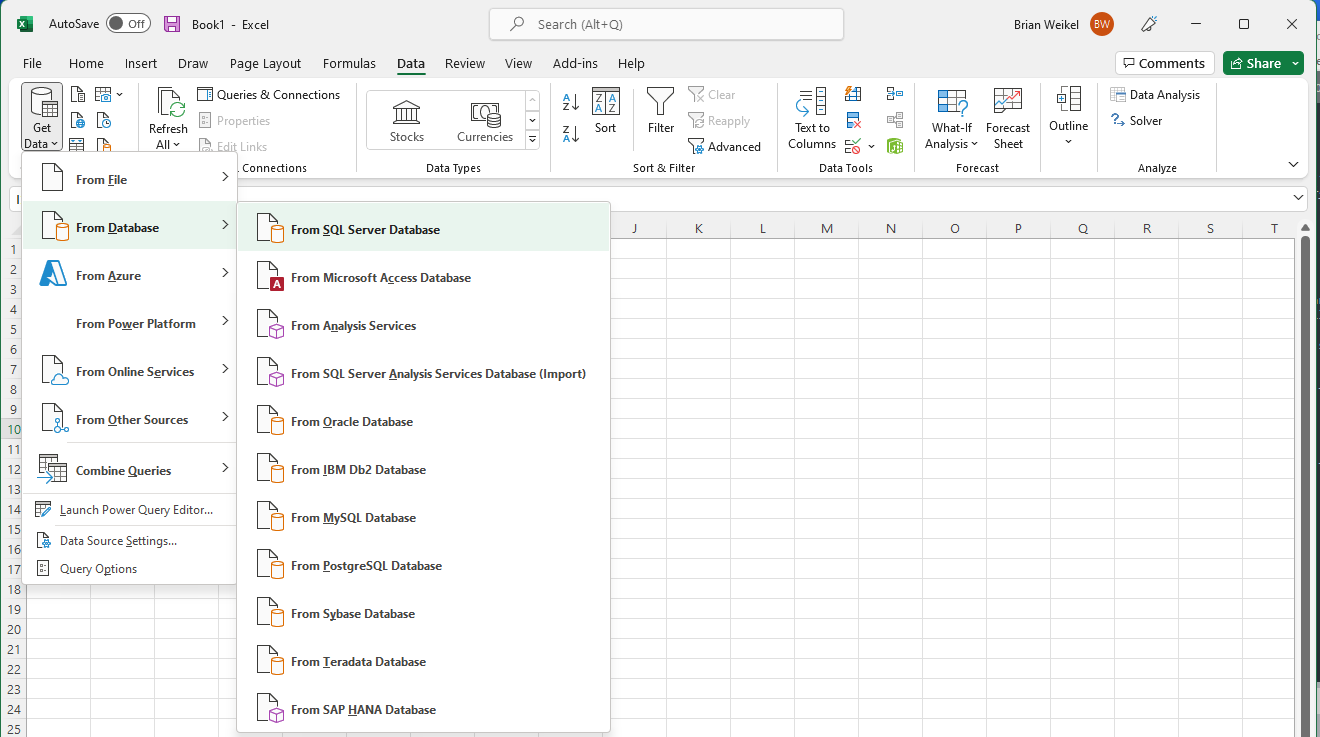
\includegraphics[height=2in, trim=0.0cm 0.0cm 0.0cm 0.0cm width=6in]{Images/Excel_2.png}
  \caption{Figure {\color{franklinblue} 2}: Excel \texttt{From Database} Options}
\end{figure}
\vspace{-1.5ex}
\small
Options include (unsurprisingly) \texttt{SQL Server Database}, (unsurprisingly) \texttt{Microsoft Access Database}, \texttt{Oracle Database}, \texttt{IBM Db2 Database}, \texttt{Teradata Database}, and \texttt{SAP Hana Database}. 
\end{frame}

\begin{frame}[t]{Excel \texttt{Data} $\rightarrow$ \texttt{Get Data} $\rightarrow$ \texttt{From Azure} Options}
\begin{figure}[htbp]
  \captionsetup{justification=centering}
  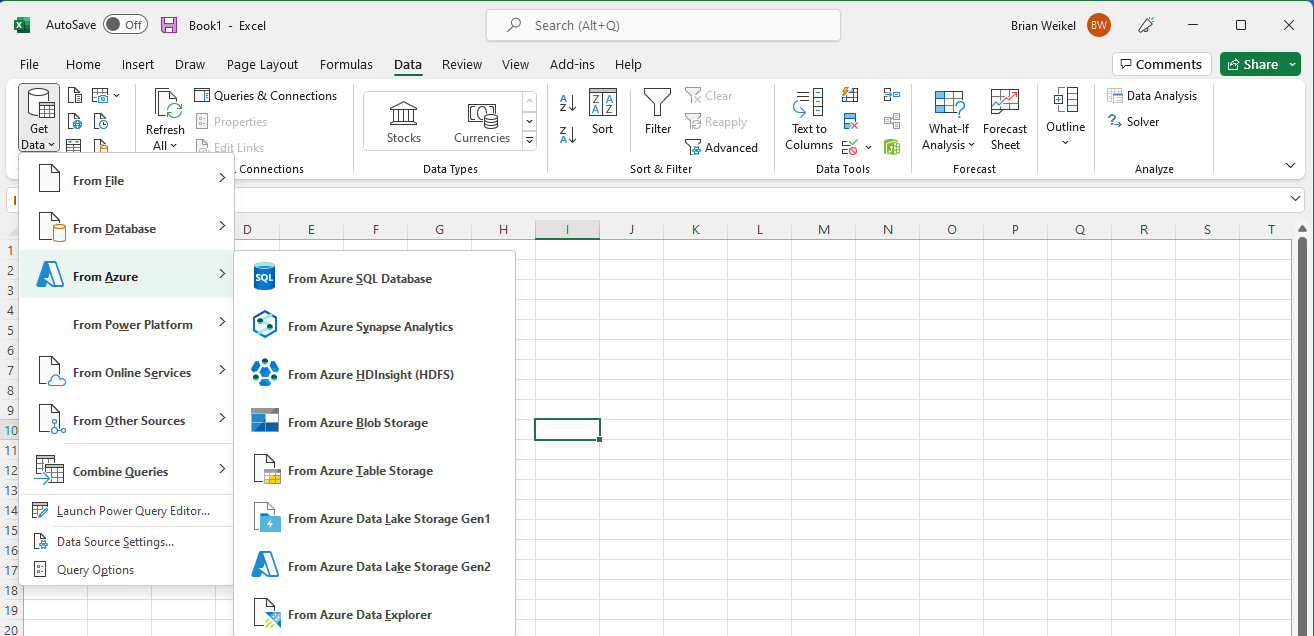
\includegraphics[height=1.7in, trim=0.0cm 0.0cm 0.0cm 0.0cm width=6in]{Images/Excel_3.png}
  \caption{Figure {\color{franklinblue} 3}: Excel \texttt{From Azure} Options}
\end{figure}
\vspace{-1.5ex}
\small
Options include \texttt{Azure SQL Database}, \texttt{Azure Blob Storage}, and several \texttt{Azure Data Lake Storage} generations.  Though not ideal from an automated, scalable, and integrated pipeline process perspective, one can use Microsoft Query to import Amazon S3 data into Excel. See \href{https://www.cdata.com/kb/tech/amazons3-odbc-excel-query.rst}{this page} for an Open Database Connectivity (OCBC) approach. 
\end{frame}

\begin{frame}[t]{Data Transformation}
Spreadsheets, along with several programming language reviewed later in these notes, can be used to:\footnote{Additional information on appropriate transformations of data indifferent to the tool used may be found in \cite{burke2021}.} \\
\vspace{2.5ex}
%https://tex.stackexchange.com/questions/228271/creating-two-columns-in-beamer
\begin{columns}[T]
\begin{column}{0.5\textwidth}
  \begin{itemize}
    \item Impute missing data.
     \vspace{1.0ex}
    \item Identify extreme outliers.
     \vspace{1.0ex}
    \item Resolve erroneous value formats.
     \vspace{1.0ex}
    \item Recognize impossible values.
      \vspace{0.0ex}
    \item Map text to numbers. 
  \end{itemize}
\end{column}
\begin{column}{0.5\textwidth}  %%<--- here
  \begin{itemize}
    \item Conduct basic content analysis.
     \vspace{1.0ex}
    \item Complete data integration.
     \vspace{1.0ex}
    \item Remediate inconsistent variable values.
     \vspace{1.0ex}
    \item Resolve duplicate records when appropriate.
  \end{itemize}  
\end{column}
\end{columns}
\end{frame}

\begin{frame}[t]{Issues Resulting from Missing Data}
\empr{Missing values} means that some values exist and others do not exist for the \textit{same row} of data. \\
\vspace{1.5ex}
Missing data may seriously compromise inference from randomized experimental designs and observational data, especially if the missing data are not handled appropriately. \\
\vspace{1.5ex} 
The potential bias due to missingness depends on the mechanism causing the data to be missing, and the methods used to ameliorate the consequences of missing data. \\ 
\vspace{1.5ex}
Missing data also adversely affects supervised and unsupervised learners, primarily by reducing prediction and classification accuracy and/or precision.\footnote{For a review of metrics for multi-class classification, see \cite{grandini2020}.} 
\end{frame}

\begin{frame}[t]{Three \underline{Basic} Options to Handle Missing Data}
While one should attempt to identify the missingness mechanism since it will determine the preferred mitigation method, several rather simple options are frequently used in business.\footnote{For an introduction to missing data mechanisms see \cite{jakobsen2017}.}  \\
\vspace{0.5ex}
\small
\begin{enumerate}
  \item The simplest option is to nullify the cells of missing values. This would mean blanking out an Excel cell if the value is (say) ``N/A'', or simply keeping it blank if it is already blank.
  \item The second option is to delete the entire record if there are missing values for the record.
  \item The third option is \empr{interpolation}, which is replacing the missing value with an estimate based on other records. % This would mean finding records that are meaningful and calculating a value for the missing cells based on what is likely to be true.
  One method is \empr{hot-deck imputation}, where each missing value is replaced with an observed response from a ``similar'' record.\footnote{For additional information on hot-deck imputation see \cite{andridge2010}.  The section \textit{Missing Data} of \cite{burke2021c} briefly reviews more advanced techniques to handle missingness.}
\end{enumerate}
\end{frame}

\begin{frame}[t]{A Simple Method to Access Missingness}
To assess the impact of deleting records with missing data one may conduct a simple analysis of a variable with missingness by examining a summary statistic of a variable that does not have missingness. \\
\vspace{1.5ex}
For example, one may calculate the average of the variable with missingness for those records with missing values and calculate the average of the variable with missingness for those records without missing values, and then compare the averages. \\
\vspace{1.5ex} 
\begin{itemize}
  \item If the averages do not differ, then deleting the records with missing data may be acceptable. 
  \item If the average values differ a lot, one should collect new data or use advanced imputation techniques rather than deleting missing data.
\end{itemize}
\end{frame}

\begin{frame}[t]{A Simple Method to Access Missingness Continued}
Example:  If one is concerned about whether records with missing gender versus records without missing gender have different purchase patterns, one can simply compare the average purchase patterns for missing versus non-missing gender records. \\
\vspace{1.5ex}
\begin{itemize}
\item If the averages are significantly different, then the missing data are concerning enough that one consider collecting new data or using more advanced imputation methods. 
\item If the averages are not significantly, then many would feel comfortable deleting the records with missing data since missing versus non-missing observations do not seem to matter in terms of purchases.
\end{itemize}
\end{frame}

\begin{frame}[t]{Outliers}
\empr{Outliers} are those data points that differ noticeably from the other data points. \\
\vspace{1.5ex}
Quartiles may be used to identify outliers. \\
\vspace{1.5ex}
\begin{enumerate}
\item The \empr{first quartile}, typically denoted $Q_1$, separates the smallest 25\% of the data from the largest 75\%. 
\item The \empr{second quartile}, typically denoted $Q_2$, separates the smallest 50\% of the data from the largest 50\%. $Q_2$ is the same as the \empr{median}. 
\item The \empr{third quartile}, typically denoted $Q_3$, separates the smallest 75\% of the data from the largest 25\%.
\end{enumerate}
\end{frame}

\begin{frame}[t]{Interquartile Range Method for Outlier Detection}
The \empr{interquartile range} (IQR) is frequently used to identify outliers.  IQR is equal to subtracting the first quartile from the third quartile.  \\
\vspace{1.5ex}
The \empr{IQR method} for detecting outliers is: \\
\vspace{1.5ex}
\begin{itemize}
  \item Compute the lower outlier boundary:  $O_L = Q_1 - 1.5 \times \text{IQR}$.
  \item Compute the upper outlier boundary:  $O_U = Q_3 + 1.5 \times \text{IQR}$.
  \item Any data value that is less than $O_L$ or greater than $O_U$ is considered to be an outlier.
\end{itemize}
\normalsize
While the IQR method typically works well in practice, other methods exist.\footnote{For a survey of methods, see \cite{aguinis2013}.}
\end{frame}

\begin{frame}[t]{IMDb Data}
\href{https://www.imdb.com/}{IMDb}, launched online in 1990 and now a subsidiary of Amazon since 1998, is the world's most popular source for movie, TV, and celebrity content.  It was designed to help fans explore the world of movies and shows, and decide what to watch. \\
\vspace{1.5ex}
IMDb offers subsets of their data  to customers for personal and non-commercial use. While you can hold local copies of the data, it is subject to their terms and conditions.\footnote{Given we will only be using the data for personal class purposes (i.e., not for commercial use), we are in compliance with their Non-Commercial Licensing and \href{https://www.imdb.com/conditions?pf_rd_m=A2FGELUUNOQJNL&pf_rd_p=3aefe545-f8d3-4562-976a-e5eb47d1bb18&pf_rd_r=F27NY89W6WHX7CDGGP5S&pf_rd_s=center-1&pf_rd_t=60601&pf_rd_i=interfaces&ref_=fea_mn_lk2}{copyright/license} agreements.} 
\\
\vspace{1.5ex}
This \href{https://www.imdb.com/interfaces/}{page} identifies data location, and the details of each provided data set.  Information provided for each data set includes variable names, variable types (e.g., string), and variable descriptions. 
\end{frame}

\begin{frame}[t]{Excel Boxplot with Outlier Detection}
\begin{figure}[htbp]
    \centering
    \captionsetup{justification=centering}
    %\fbox{\includegraphics[trim=0cm 9cm 0cm 9cm]{C:/Users/bkwei/OneDrive - Franklin University/Desktop/Math_215/LaTeX_Modules/startYear_frequency_distr2.pdf}}  
    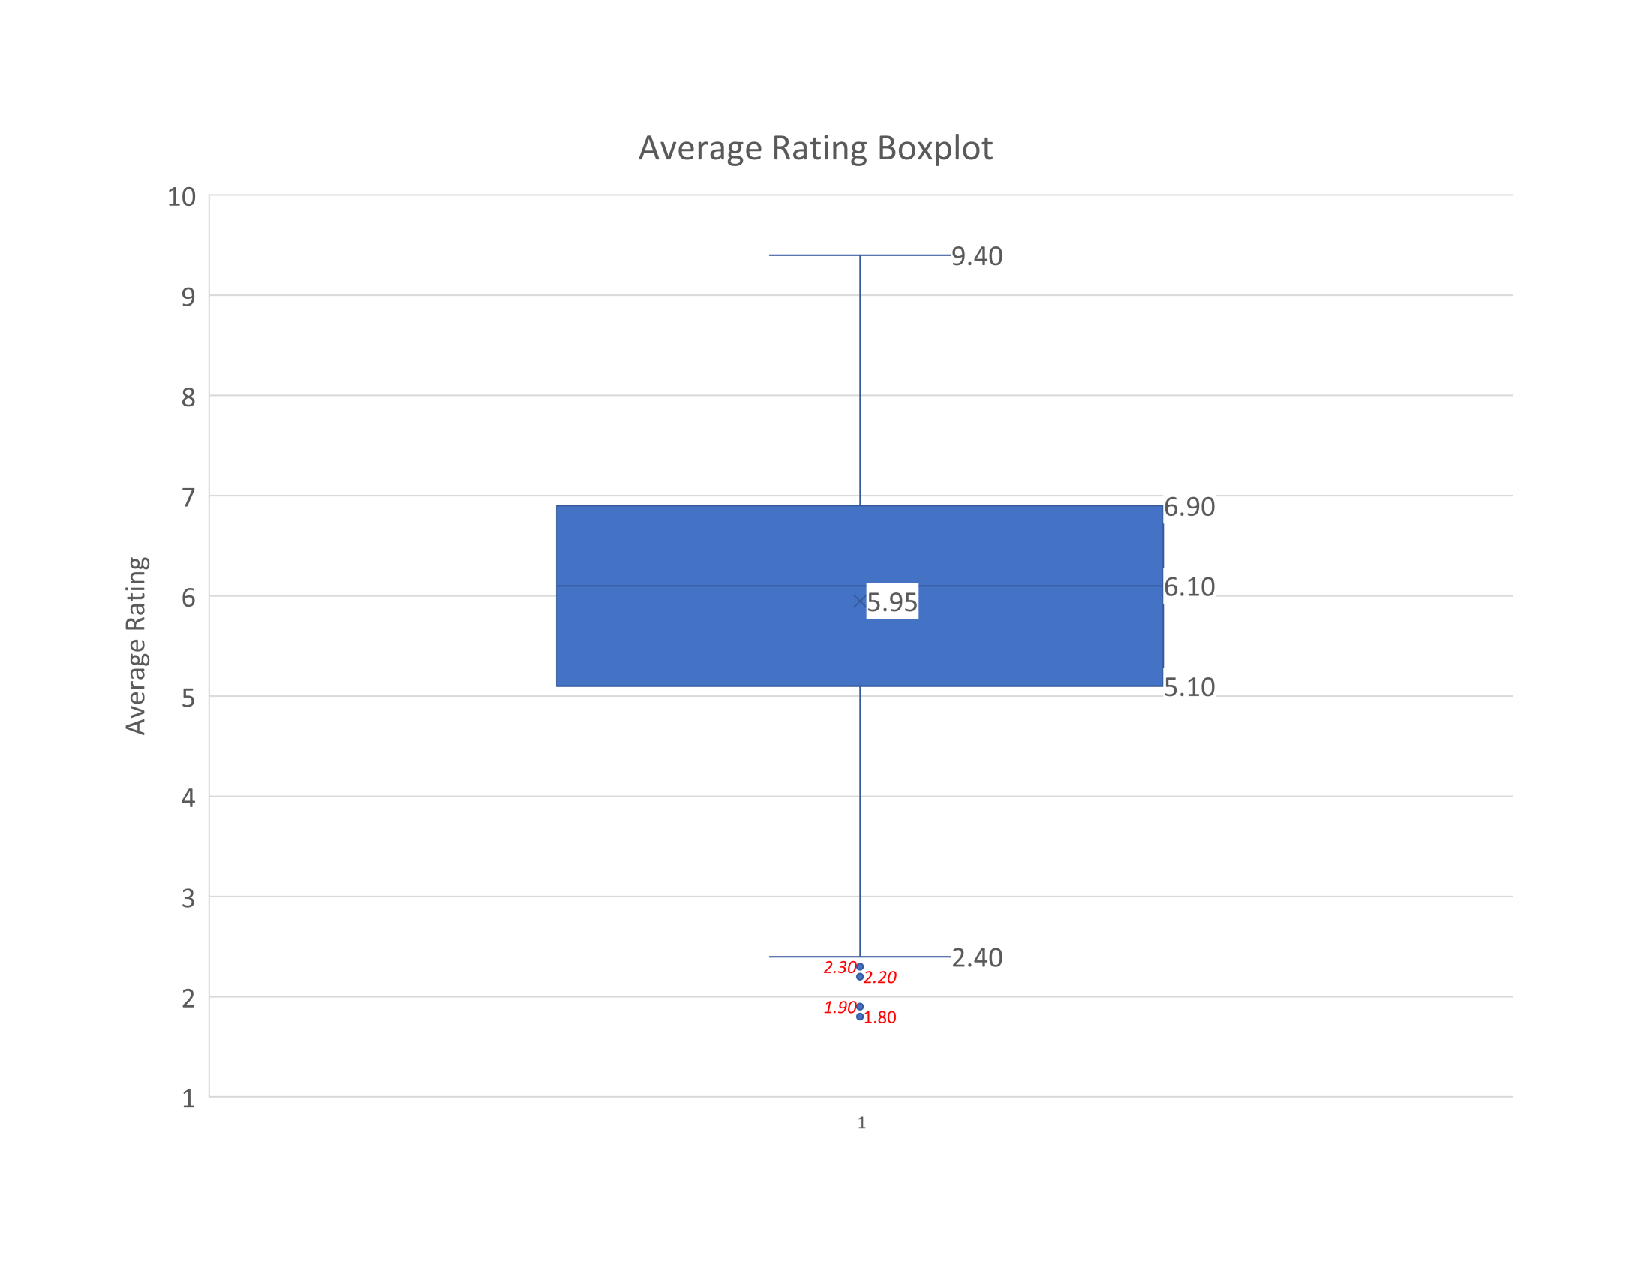
\includegraphics[clip, trim=0cm 2.3cm 0cm 2.3cm, width=0.7\textwidth]{Images/averageRating_Boxplot.pdf}  
    \caption{Figure 4: Average Rating Boxplot}
    \label{fig:arboxplot}
\end{figure}
\vspace{-2.0ex}
\small
In Figure \ref{fig:arboxplot}, $Q_1$, $Q_2$, $Q_3$, the sample mean (i.e., 5.95), the maximum, and a \underline{local} \underline{minimum} are shown for IMDb Movie Average Ratings for movies released between 2017 and 2021. Any value less than 2.4 is considered an outlier by Excel;  outliers are shown in \emph{\textcolor{red}{red font}}.  Dependent on the data, Excel may show a \underline{local} \underline{maximum} in lieu of the maximum.\\
\end{frame}

\begin{frame}[t]{Erroneous Value Formats and Impossible Values}
\empr{Erroneous value formats} are typically words that are meant to be numbers. For example the number of days since last purchase is recorded as ``two hundred'' in lieu of 200. \\
\vspace{1.5ex} 
 \empr{Impossible values} are similar to outliers: they do not belong in the range of acceptable values. For example if the number of days since last purchase, relative to the current date, is 365,000 or -100 there is no need to use the IQR method to determine if the values are extreme; the data are obviously wrong.\\
\vspace{1.5ex}
Many times, data is not in a numerical format. For example the values for a column of data called Gender may be ``Female'', ``Male'', ``Other'', or ``Unknown''. Thus the variables would need to be mapped to categorical variables or indicator variables (e.g., dummy variables).  As a case in point let the variable $X1$ be defined as 1 if Gender is Female, and 0 otherwise.
\end{frame}

\begin{frame}[t]{Content Analysis}
Narrowly defined, \empr{content analysis} is the examination of digital text, photos, audio, or visual formats of communication, which may or may not be extracted from social media. More generally, content analysis includes the careful examination of face-to-face human interactions, analysis of character portrayals in media venues ranging from novels to online videos, computer-driven analysis of word usage in news media and political speeches, advertising, and blogs, examination of interactive content such as video gaming and social media exchanges, and much more.\footnote{For an introduction to content analysis, see \cite{krippendorff2019}.} % More generally, content analysis is the systematic, objective, quantitative analysis of message  characteristics. It includes both human-coded analyses and computer-aided text analysis (CATA).
 \\
\vspace{1.5ex}
Another way to deal with text is to count the number of times a word appears, a basic form of content analysis. This can be done as an analysis for the entire data spreadsheet; such as counting the unique instances of ``Female'', ``FEMALE'', ``female'', ``Male'', ``MALE'', ``male'', \ldots for the variable Gender.    
\end{frame}

\begin{frame}[t]{Data Integration}
Data transformation frequently includes integrating two sources of data. While we will soon cover more advanced ways of doing this task with programming languages, such as with Python or structured query language (SQL) for relational databases, Excel can be used to accomplish a few basic integration tasks. \\
\vspace{1.5ex}
\begin{itemize}
\item Excel offers a way to connect data in two spreadsheets with the \href{https://support.microsoft.com/en-us/office/vlookup-function-0bbc8083-26fe-4963-8ab8-93a18ad188a1}{VLOOKUP} function. 
\item Another useful Excel data integration option is the \href{https://support.microsoft.com/en-us/office/match-function-e8dffd45-c762-47d6-bf89-533f4a37673a}{MATCH} function.
\end{itemize}
\end{frame}

\section{Programming Tools}

\begin{frame}[t]{Programming and Programming Language Defined}

\empr{Programming} is the process of solving a problem using computer algorithms. A \empr{computer algorithm} is a well-defined procedure that allows a computer to solve a problem.  \empr{Statistical programming} is the process of solving \textit{data-related} problems using executable computer algorithms. \\
\vspace{1.5ex}
A \empr{programming language} is a formal set of instructions that can be used to produce various kinds of data output. \\
\vspace{1.5ex}
\begin{columns}[T]
\begin{column}{0.2\textwidth}
\begin{figure}[htbp]
  \captionsetup{justification=centering}
  
\includegraphics[height=0.8cm, trim=0.1cm 0.1cm 0.1cm 0.1cm width=0.75cm]{Images/Python.png}
  %\caption{Figure {\color{franklinblue} 1}:}
\end{figure} 
\end{column}
\begin{column}{0.7\textwidth}  %%<--- here
\href{https://www.python.org/}{Python} is an interpreted, object-oriented, high-level programming language with dynamic semantics. Its high-level built in data structures, combined with dynamic typing and dynamic binding, make it very attractive for rapid application development, as well as for use as a scripting or glue language to connect existing components together. 
\end{column}
\end{columns}
\end{frame}

\begin{frame}[t]{R and SQL}
\begin{columns}[T]
\begin{column}{0.2\textwidth}
\begin{figure}[htbp]
  \captionsetup{justification=centering}
  
\includegraphics[height=1.0cm, trim=0.1cm 0.1cm 0.1cm 0.1cm width=1.0cm]{Images/R.jpg}
  %\caption{Figure {\color{franklinblue} 1}:}
\end{figure}
\end{column}
\begin{column}{0.7\textwidth}  %%<--- here
\href{https://www.r-project.org/about.html}{R} is a language and environment for statistical computing and graphics.  It is a \href{https://www.gnu.org/gnu/thegnuproject.html}{GNU project}. R is similar to the \href{https://web.archive.org/web/20181014111802/http://ect.bell-labs.com/sl/S/}{S language and environment} which was developed at Bell Laboratories (formerly AT\&T, now Lucent Technologies) in the 1970's by John Chambers and colleagues. \\
\vspace{1.5ex}
\empr{Structured Query Language}, or simply \empr{SQL} is a domain-specific language designed for managing data held in a relational database management system (RDBMS), or for stream processing in a relational data stream management system (RDSMS). %It is particularly useful in handling structured data.
\end{column}
\end{columns}
\vspace{0.0ex} 
While the most popular languages for marketing analytics and data science are Python and R, other languages  one will encounter include \href{https://julialang.org/}{Julia} and \href{https://www.scala-lang.org/}{Scala}. 
\end{frame}

\begin{frame}[t]{Defining Programming Tool, Code and Software}
A \empr{programming tool} is a software package that allows for the execution of a programming language. A \empr{statistical programming tool} is a programming tool focused on statistical analyses of data. \\
\vspace{1.5ex}
\empr{Programming code} are statements written in a particular programming language. \\
\vspace{1.5ex}
\empr{Programming software for data} is a set of specialized computer programs for analysis using programming code.\\
\vspace{1.5ex}
\empr{Non-programming software for data} is a set of specialized computer programs for analysis using a graphical interface.
\vspace{1.5ex}
\end{frame}

\begin{frame}[t]{Excel versus Programming Tools, like R and Python}
Excel Advantages \\
\vspace{0ex}
\small
\begin{itemize}
  \item It is easier to get started and learning resources are rich.
  \item Has many built-in easy-to-use functions. 
  \item Can assist in understanding many operations available in R and Python.  
\end{itemize}
\vspace{-1.5ex}
\normalsize
Excel Disadvantages \\
\vspace{0ex}
\small
\begin{itemize}
  \item Has limited advanced statistics (even with \href{https://learn.microsoft.com/en-us/office/dev/add-ins/excel/excel-add-ins-overview}{add-ins}).
  \item To fully master Excel you need to learn \href{https://learn.microsoft.com/en-us/office/vba/library-reference/concepts/getting-started-with-vba-in-office}{VBA}, which has more limited capabilities than R and Python. 
  \item The Excel data file can only hold 1.08 million rows sans the aid of other tools, and its not suitable for processing large-scale data sets.
  \item Unlike R and Python, there is a fee for Excel.\footnote{\href{https://www.google.com/sheets/about/}{Google Sheets} does not charge a fee for tool use.}
\end{itemize}
\end{frame}

\begin{frame}[t]{Comparing R and Python}
% https://www.educba.com/r-vs-python/
% https://www.esparkinfo.com/blog/r-vs-python.html
\begin{enumerate}
  \item Python is a general purpose language (GPL). R is a domain-specific language (DSL). 
  \item Python has more big-data supervised (e.g., deep learning), unsupervised learning, and scientific computation capabilities, and data handling modules:  \href{https://numpy.org/}{Numpy}, \href{https://scipy.org/}{SciPy}, \href{https://scikit-learn.org/stable/}{scikit-learn}, \href{https://www.sympy.org/en/index.html}{SymPy}, \href{https://pandas.pydata.org/}{Pandas} \ldots. 
  \item R has more statistics and econometric packages available for immediate use. 
  \item While R and Python both have many graphical techniques, R graphics tend to be more elegant and  visually appealing. 
\end{enumerate}
\end{frame}

 \begin{frame}[t]{Comparing R and Python Continued}
 \begin{enumerate}
 \setcounter{enumi}{4}
   \item R has many \href{https://cran.r-project.org/}{packages}, about 19,000, where some accomplish the same task.  Python is designed on the \href{https://peps.python.org/pep-0020/}{philosophy} that ``there should be one and preferably only obvious way to do it.'' 
  \item Python is typically easier to learn than R.  However, learning Python libraries can be a bit complex relative to learning R libraries and plots.
  \item R is slower than Python, but not by much.
  \item Python is more popular than R, particularly so in business software engineering (SE) departments.
\end{enumerate}
\end{frame}

\begin{frame}[t]{Integrated Development Environments for Python}
Popular integrated development environments (IDEs) used for Python include: \\
\vspace{1.5ex}
\begin{columns}[T]
\begin{column}{0.2\textwidth}
\begin{figure}[htbp]
  \captionsetup{justification=centering}
  
\includegraphics[height=1.2cm, trim=0.1cm 0.1cm 0.1cm 0.1cm width=1.2cm]{Images/PyCharm.jpg}
  %\caption{Figure {\color{franklinblue} 1}:}
\end{figure}
\end{column}
\begin{column}{0.7\textwidth}  %%<--- here
\href{https://www.jetbrains.com/pycharm/}{PyCharm} provides code analysis, a graphical debugger, an integrated unit tester, integration with version control systems, and supports web development with \href{https://www.djangoproject.com/}{Django}. PyCharm is developed by the Czech company \href{https://www.jetbrains.com/}{JetBrains}. \\
\vspace{1.5ex}
The textbook mentions \href{https://github.com/yhat/rodeo}{Rodeo}, which is is an open-source IDE that is lightweight and customizable. 
\end{column}
\end{columns}
\vspace{1.5ex}
Caution is advised about using Rodeo as an IDE.  The linked Github repository has not been updated in years.  Thus the code base does not appear to be actively maintained.\footnote{Neither I nor anyone I know has ever used Rodeo.}
\end{frame}

\begin{frame}[t]{Jupyter Products}
\begin{columns}[T]
\begin{column}{0.2\textwidth}
\begin{figure}[htbp]
  \captionsetup{justification=centering}
  
\includegraphics[height=1.2cm, trim=0.1cm 0.1cm 0.1cm 0.1cm width=1.2cm]{Images/Juypter.png}
  %\caption{Figure {\color{franklinblue} 1}:}
\end{figure}
\end{column}
\begin{column}{0.7\textwidth}  %%<--- here
The classic \href{https://jupyter.org/}{Jupyter Notebook} is the original web application for creating and sharing computational documents. The open source web application offers a simple, streamlined, document-centric experience. \\
\vspace{1.5ex}
\href{http://jupyter.org/try}{JupyterLab} is the latest web-based interactive development environment for notebooks, code, and data. Its flexible interface allows users to configure and arrange workflows in data science, scientific computing, computational journalism, and machine learning. A modular design invites extensions to expand and enrich functionality.
\end{column}
\end{columns}
The name ``Jupyter'' comes from the core supported programming languages that it supports: Julia, Python, and R.%\footnote{%Jupyter Notebooks are a spin-off project from the IPython project, which at one time had a IPython Notebook. 
%A Jupyter Notebook is the application where I have done much of my Python data science development.}
\end{frame}

\begin{frame}[t]{Juypter Notebook}
\begin{figure}[htbp]
  \captionsetup{justification=centering}
  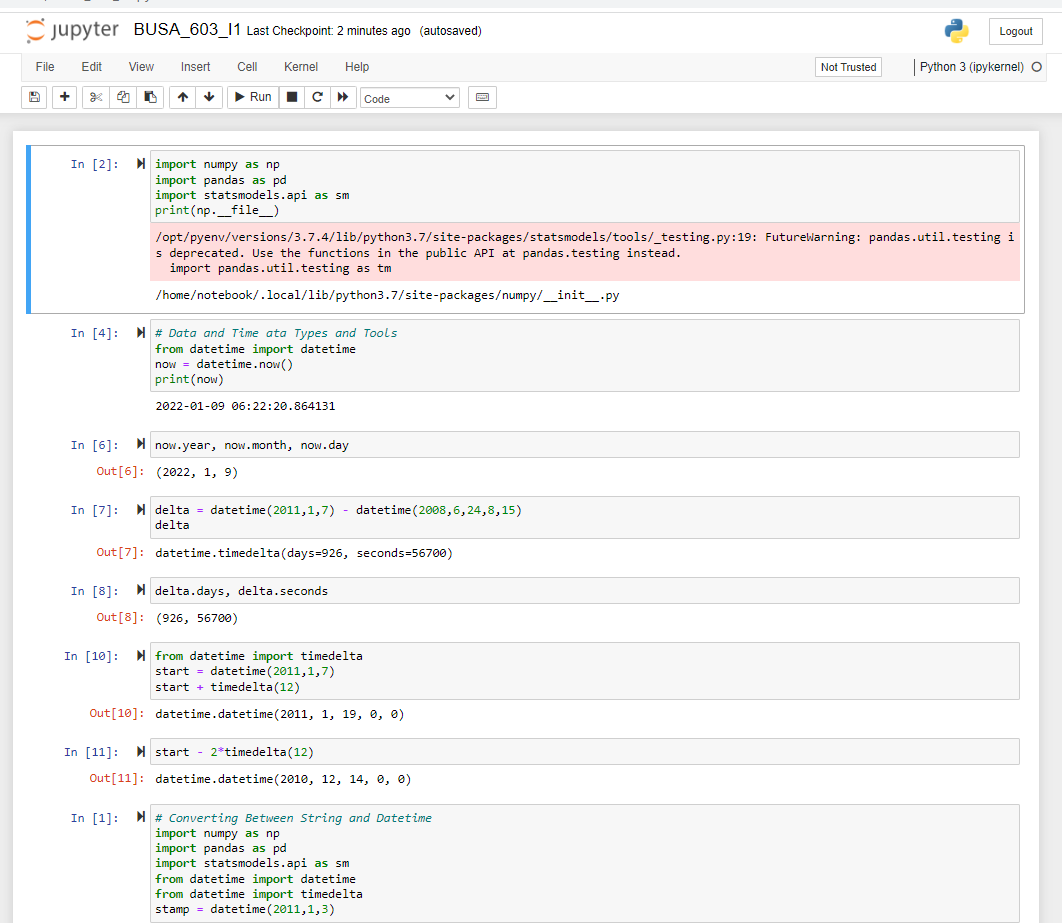
\includegraphics[height=7cm, trim=0.0cm 0.0cm 0.0cm 0.0cm width=7cm]{Images/Jupyter_Python.png}
  \caption{Figure {\color{franklinblue} 5}: Juypter Notebook with Python Executable Code}
\end{figure}
\end{frame}

\begin{frame}[t]{An R IDE and the Sublime Text Editor}
\begin{columns}[T]
\begin{column}{0.2\textwidth}
\begin{figure}[htbp]
  \captionsetup{justification=centering}
  
\includegraphics[height=1.2cm, trim=0.1cm 0.1cm 0.1cm 0.1cm width=1.2cm]{Images/R.jpg}
  %\caption{Figure {\color{franklinblue} 1}:}
\end{figure}
\vspace{8.0ex}
\begin{figure}[htbp]
  \captionsetup{justification=centering}
  
\includegraphics[height=1.2cm, trim=0.1cm 0.1cm 0.1cm 0.1cm width=1.2cm]{Images/Sublime_Text.jpg}
  %\caption{Figure {\color{franklinblue} 1}:}
\end{figure}
\end{column}
\begin{column}{0.7\textwidth}  %%<--- here
\href{https://posit.co/download/rstudio-desktop/}{RStudio} is an open source IDE for R. It is available in two formats: RStudio Desktop is a desktop application while RStudio Server runs on a remote server and allows accessing RStudio using a web browser. \\
\vspace{1.5ex}
\href{https://www.sublimetext.com/}{Sublime Text} is one of the most popular text editors in the world. It has many powerful features like multi-line editing, build systems for dozens of programming languages, regex find and replace, a Python API for developing plugins, and more.  In addition, it is cross-platform (i.e., Mac, Windows, and Linux), and it is distributed as ``shareware''; thus it is free to use with the occasional purchase pop-up.
\end{column}
\end{columns}
\end{frame}

\begin{frame}[t]{RStudio}
\begin{figure}[htbp]
  \captionsetup{justification=centering}
  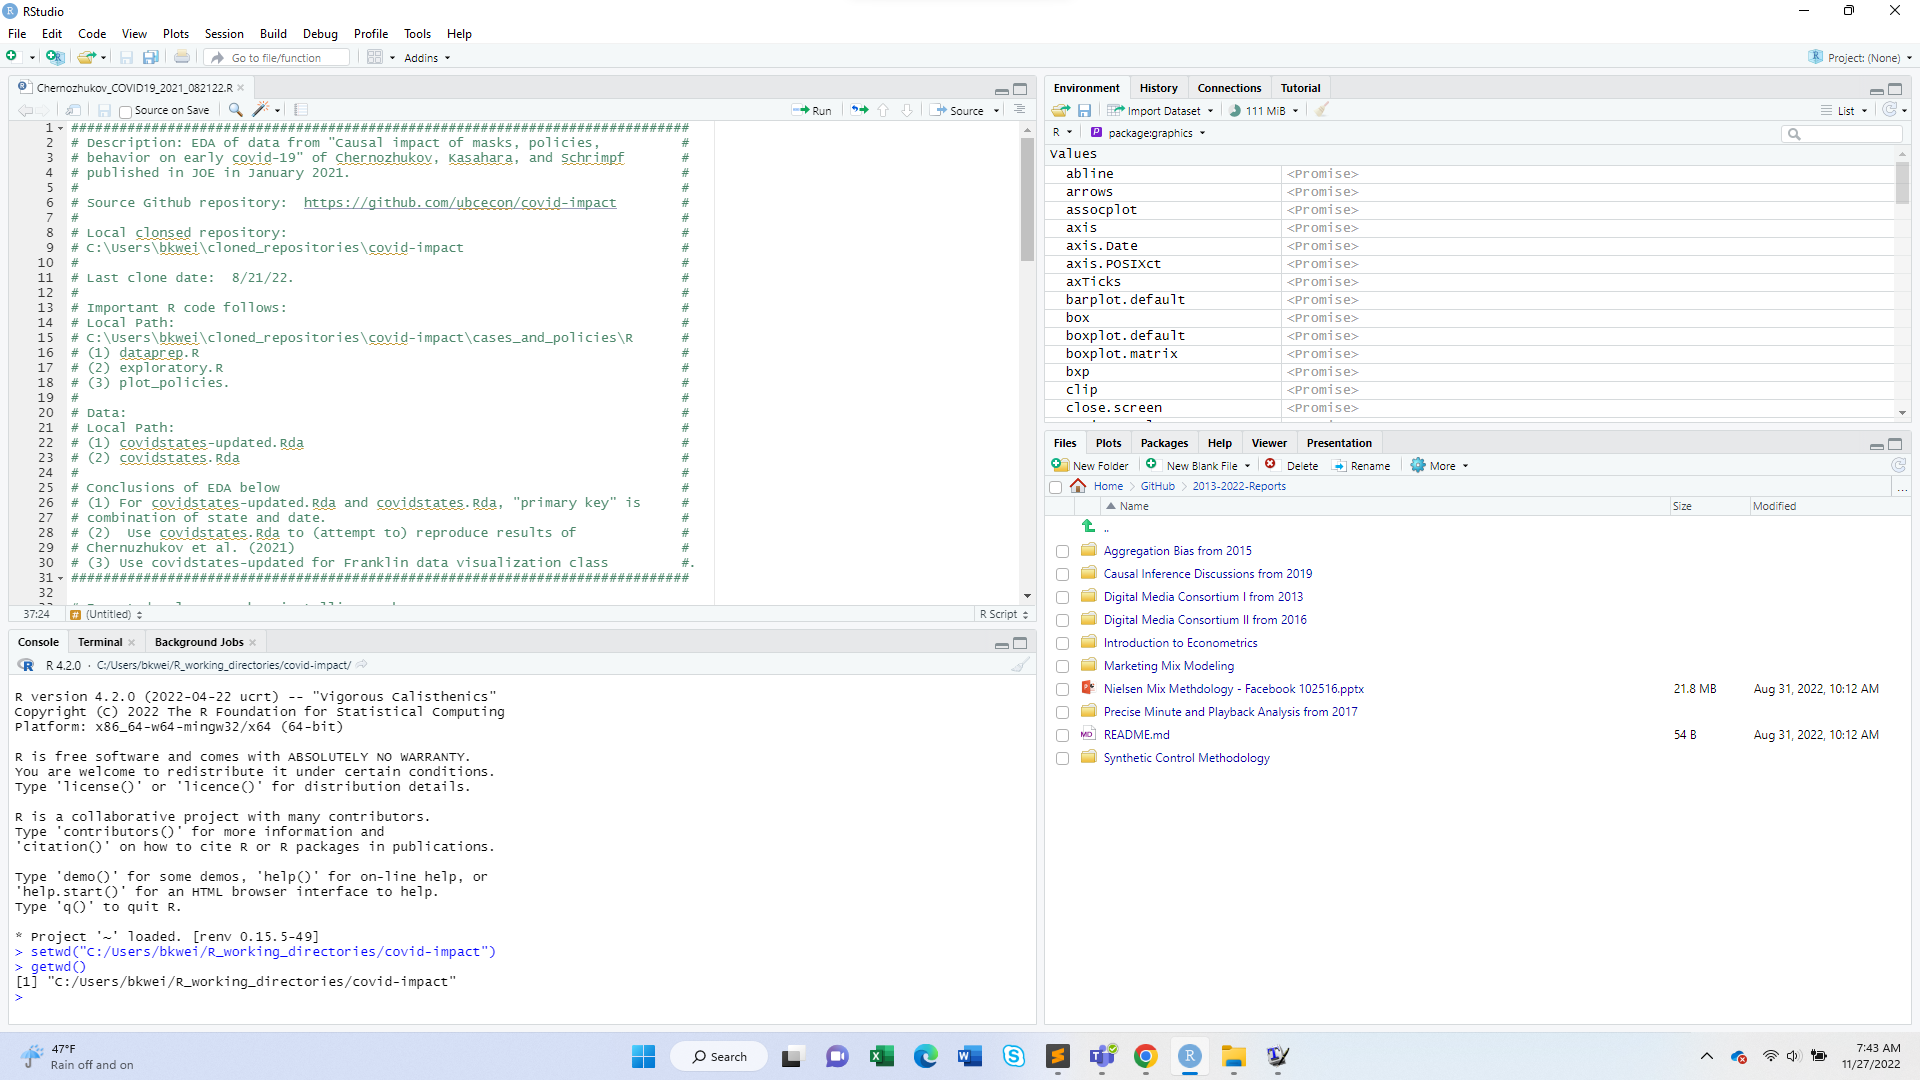
\includegraphics[height=6cm, trim=0.0cm 0.0cm 0.0cm 0.0cm width=6cm]{Images/R_Console.png}
  \caption{Figure {\color{franklinblue} 6}: RStudio }
\end{figure}
\end{frame}

\begin{frame}[t]{Orchestration}
\begin{columns}[T]
\begin{column}{0.2\textwidth}
\begin{figure}[htbp]
  \captionsetup{justification=centering}
  \includegraphics[height=0.9cm, trim=0.1cm 0.1cm 0.1cm 0.1cm width=0.9cm]{Images/Apache_AirFlow.png}
  %\caption{Figure {\color{franklinblue} 1}:}
\end{figure}
\vspace{13.0ex}
\begin{figure}[htbp]
  \captionsetup{justification=centering}
  
\includegraphics[height=0.9cm, trim=0.1cm 0.1cm 0.1cm 0.1cm width=0.9cm]{Images/Luigi.png}
  %\caption{Figure {\color{franklinblue} 1}:}
\end{figure}
\end{column}
\begin{column}{0.7\textwidth}  %%<--- here
\href{https://airflow.apache.org/}{Apache Airflow} is an open-source platform for developing, scheduling, and monitoring batch-oriented workflows via a web interface, where its extensible Python framework enables one to build workflows connecting with virtually any technology. %A web interface helps manage the state of your workflows. 
%It can be deployed from a single process on a laptop to a distributed setup to support large workflows. %Airflow is deployable in many ways, varying from a single process on your laptop to a distributed setup to support even the biggest workflows. %\href{https://airflow.apache.org/docs/apache-airflow/stable/concepts/dags.html}{Directed acyclic graphs} (DAGs) are the foundation of its workflow.
\\
\vspace{1.5ex}
\href{https://luigi.readthedocs.io/en/stable/index.html}{Luigi} is a Python (2.7, 3.6, 3.7 tested) package that helps one build pipelines of batch jobs. It handles dependency resolution, workflow management, visualization, handling failures, and command line integration.
\end{column}
\end{columns}
Airflow tends to be the orchestrating workflow choice for many SE departments.\footnote{The Appendix provides additional information on the architecture of Airflow.}
\end{frame}

\begin{frame}[t]{Repositories}
\begin{columns}[T]
\begin{column}{0.2\textwidth}
\begin{figure}[htbp]
  \captionsetup{justification=centering}
  
\includegraphics[height=1.2cm, trim=0.1cm 0.1cm 0.1cm 0.1cm width=1.2cm]{Images/Github.png}
  %\caption{Figure {\color{franklinblue} 1}:}
\end{figure}
\vspace{12.0ex}
\begin{figure}[htbp]
  \captionsetup{justification=centering}
  
\includegraphics[height=0.9cm, trim=0.1cm 0.1cm 0.1cm 0.1cm width=0.9cm]{Images/Gitlab.png}
  %\caption{Figure {\color{franklinblue} 1}:}
\end{figure}
\end{column}
\begin{column}{0.7\textwidth}  %%<--- here
\href{https://github.com/}{GitHub} is an online software development platform. It's used for storing, tracking, and collaborating on software projects. It provides the distributed version control of Git plus access control, bug tracking, software feature requests, task management, continuous integration, and wikis for every project.%\footnote{I use Github as a repository for my code.}
 \\
\vspace{1.5ex}
\href{https://about.gitlab.com/}{GitLab} is a DevOps software package that combines the ability to develop, secure, and operate software in a single application.  Due to its ever expanding capabilities and support, it is typically favored by SE departments.  
\end{column}
\end{columns}
\end{frame}

\section{Variables and Variable Types}

\begin{frame}[t]{Variables and Variable Types}
Excel, R, and Python use variables. \\
\vspace{1.5ex}
A \empr{variable} is a storage mechanism for a particular identifier, which contains information referred to as a \empr{value}. \\
\vspace{1.5ex}
A variable is like a column of data, and a variable's response values are like rows of data in an Excel spreadsheet, or a \empr{data frame} in R.\footnote{A data frame is a generic R data object, which are used to store tabular data. One may use the Pandas package to create data frames in Python.}  \\
\vspace{1.5ex} 
A \empr{data set} is a collection of related sets of information that is composed of separate elements but can be manipulated as a unit by a computer.  A data frame and an Excel spreadsheet may both be considered a data set.
\end{frame}

\begin{frame}[t]{A Data Set Example}
\scriptsize
\begin{table}[h!]
\begin{center}
\begin{tabular}{L{2.2cm} L{0.8cm} L{0.8cm} L{1.5cm} L{2.8cm}} 
%\hline
\texttt{Name} &  \texttt{HT} & \texttt{WT} & \texttt{Birth\_Date} & \texttt{Birth\_Place} \\
\midrule  
  Jet Greaves & 6'0'' & 184 & 3/30/01 & Cambridge, ON, CAN \\
  Nolan Lalonde & 6'1'' &  190 & 2/14/04 & Kingston, ON, CAN \\
  Elvis Merzlikins & 6'3'' & 183  & 4/13/94 & Riga, LVA \\
  Daniil Tarasov & 6'5''  & 196 & 3/27/99 & Novokuznetsk, RUS \\
 \midrule
\end{tabular}
\caption{\label{tab:TE}Tender Employees}
\end{center}
\end{table}
\small
\vspace{-1ex}
Some basic features are found in most structured data sets. Information is collected on \underline{individuals, households, persons, firms, animals, plants,} \underline{subjects, items, objects}, \ldots\\
\vspace{1.5ex}
 In Table \ref{tab:TE}, the information collected is on employees. %The individual characteristics are the variables.
The variables of Table \ref{tab:TE}  \texttt{Name}, \texttt{HT}, \texttt{WT}, \texttt{Birth\_Date}, and \texttt{Birth\_Place}. The values of the variables are also called \empr{data}.  \\
 \vspace{1.5ex}
 You may hear some refer to the combination of attributes that result in unique identification as \empr{records} or \empr{observations};  The variable \texttt{Name} of Table \ref{tab:TE} uniquely identifies an employee.  
\end{frame}

\begin{frame}[t]{Common Data Types}
\small
\begin{itemize}
\item \empr{Character}: the variable contains words that do not have order or numerical meaning.  Also called a \empr{string} or \empr{text variable}.  An example is \texttt{Name} of Table \ref{tab:TE}.
\item \empr{Numeric}: the variable contains numbers with decimal points.  May also be called a \empr{decimal}, \empr{real}, or \empr{float}. For example, \texttt{WT} of Table \ref{tab:TE}.
\item \empr{Integer}: the variable contains numbers without decimal points.  For example, we could use \texttt{Birth\_Date} of Table \ref{tab:TE}  to calculate an employee's age in years.
\item \empr{Logical}: the variable contains only two possible values, such as TRUE or FALSE. Also called a \empr{boolean variable}, or an \empr{indicator variable} or \empr{dummy variable} when a variable is mapped to an integer.  As an example, we may create a variable \texttt{NA\_Birth} that equals 1 if Table \ref{tab:TE}'s \texttt{Birth\_Place} country for a \texttt{Name} is in North American, and 0 otherwise.
\end{itemize}
\end{frame}

\section{First, Second and Third Party Data}

\begin{frame}[t]{Classification of Data Sources}
Marketing uses data from a variety of sources. \\
\vspace{1.5ex} 
%\small
\begin{itemize}
\item \empr{First party data} are a firm's own internal data, such as sales and customer information.
\item \empr{Second party data} are another firm's first party data, shared directly from the source. 
\item \empr{Third party data}, also called syndicated data, are also data from other firms but without a direct relationship or agreement to the customer, such as data scraped from public websites or apps, or data purchased from a provider such as, \href{https://www.iriworldwide.com/en-us}{IRI}, \href{https://www.nielsen.com/}{Nielsen}, \href{https://nielseniq.com/global/en/}{NielsenIQ}, \href{https://www.npd.com/}{NPD}, or \href{https://www.spins.com/}{Spins}.
\end{itemize}
\vspace{0.0ex}
\normalsize
The goal is to integrate first party data with second and third party data to optimize marketing outcomes. \\
\vspace{1.5ex}
\end{frame}

\section{Data Management Platforms}

\begin{frame}[t]{Inbound Marketing}
\empr{Inbound marketing} is a business methodology that attracts customers by creating valuable content and experiences tailored to them. It inspires long-term customer relationships.\\
\vspace{1.5ex}
An \empr{inbound marketing tool} is marketing software designed to help marketers manage digital content and campaigns.\\
\vspace{1.5ex}
In contrast traditional marketing strategies, such as \empr{outbound marketing}, attempt to push content to consumers to promote products and services.
\end{frame}

\begin{frame}[t]{Inbound Marketing and the Purchase Funnel}
%https://tex.stackexchange.com/questions/57418/crop-an-inserted-image
Inbound marketing attempts to make each element of the \empr{purchase funnel} larger. \\
\vspace{1.5ex}
\begin{figure}[htbp]
  \captionsetup{justification=centering}
  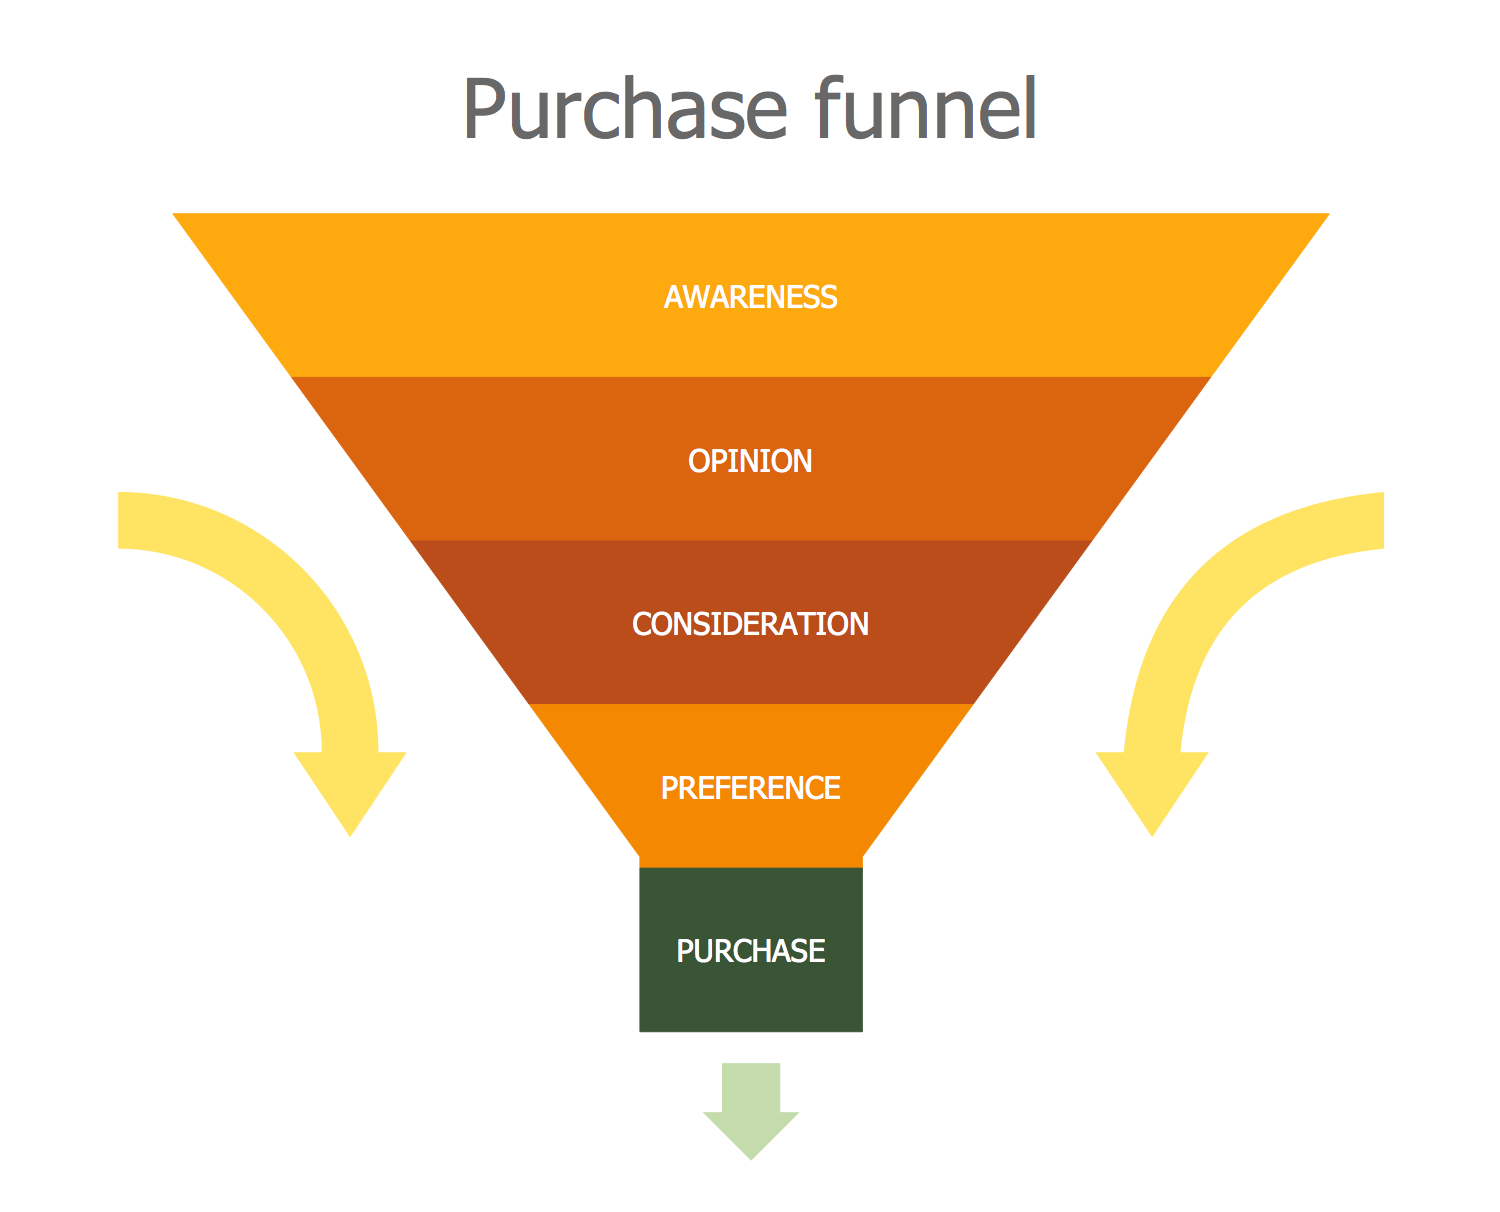
\includegraphics[height=5.6cm, trim=0.0cm 0.0cm 0.0cm 5.0cm, clip, width=8cm]{Images/Purchase_Funnel.png}
  \caption{Figure {\color{franklinblue} 7}: A Purchase Funnel}
\end{figure}
\end{frame}

\begin{frame}[t]{Inbound Marketing Media \& Tools}
Common type of inbound marketing media and/or content. \\
\vspace{2.0ex}
\begin{columns}[T]
\begin{column}{0.3\textwidth}
\begin{itemize}
\item Blog Posts
\vspace{1.0ex}
\item Guides \& E-books
\vspace{1.0ex}
\item White Papers
\vspace{1.0ex}
\item Infographics
\vspace{1.5ex}
\item Search Engine Optimization (SEO)
\end{itemize}
\end{column}
\begin{column}{0.3\textwidth} 
 \begin{itemize}
\item Inbound Email 
\vspace{1.0ex}
\item Webinars \& Podcasts
\vspace{1.0ex}
\item News Articles
\vspace{1.0ex}
\item Direct Mailers
\end{itemize} 
\end{column}
\begin{column}{0.3\textwidth} 
\begin{itemize}
\item Social Media
\vspace{1.0ex}
\item Research Reports
\vspace{1.0ex}
\item Slideshare
\vspace{1.0ex}
\item Videos 
\end{itemize}  
\end{column}
\end{columns}
Inbound marketing platforms manage digital marketing campaigns using just first party data. Inbound marketing tools include \href{https://ahrefs.com/}{Ahrefs}, \href{https://www.drift.com/}{Drift}, \href{https://www.hubspot.com/}{Hubspot}, \href{https://www.leadfeeder.com/}{Leadfeeder}, \href{https://www.marketo.com/}{Marketo}, \href{https://www.salesforce.com/}{Salesforce}, and \href{https://www.semrush.com/}{SEMRush}.
\end{frame}

\begin{frame}[t]{Data Management Platforms}
Marketers need a system to store, organize, and analyze data before it becomes useful and easily understood. A \empr{data management platform} (DMP) is such a solution. A DMP: \\
\vspace{0.0ex}
\small
\begin{itemize}
\item Collects and organizes data so marketers may target specific audiences on \empr{ad networks}.\footnote{Ad networks provide an outsourced sales capability for publishers and a means to aggregate inventory and audiences from numerous sources in a single buying opportunity for media buyers.} 
\item Measures campaign performance across segments and channels to increase marketing outcomes, such as a consumer purchase.
\item Integrates digital marketing data with non-digital data sources (i.e., second and third party data integration).
\end{itemize}
\vspace{-1.0ex}
\normalsize
Notable DMPs include \href{https://theadex.com/}{The ADEX}, \href{https://business.adobe.com/what-is-experience-cloud.html}{Adobe Cloud Experience}, \href{https://www.lotame.com/}{Lotame}, \href{https://www.home.neustar/}{Neustar}, \href{https://www.nielsen.com/solutions/media-planning/marketing-cloud/}{Nielsen Marketing Cloud}, \href{https://www.oracle.com/cx/marketing/data-management-platform/}{Oracle BlueKai}, and \href{https://www.salesforce.com/products/marketing-cloud/data-management/}{Salesforce Audience Studio}.
\end{frame}

\begin{frame}[t]{LUMAscapes}
\href{https://lumapartners.com/luma-content/\#lumascapes}{LUMA} provides a set of online maps that categorizes different entities in the digital media and marketing ecosystems. \\
\vspace{1.5ex}
\begin{figure}[htbp]
    \centering
    \captionsetup{justification=centering}
    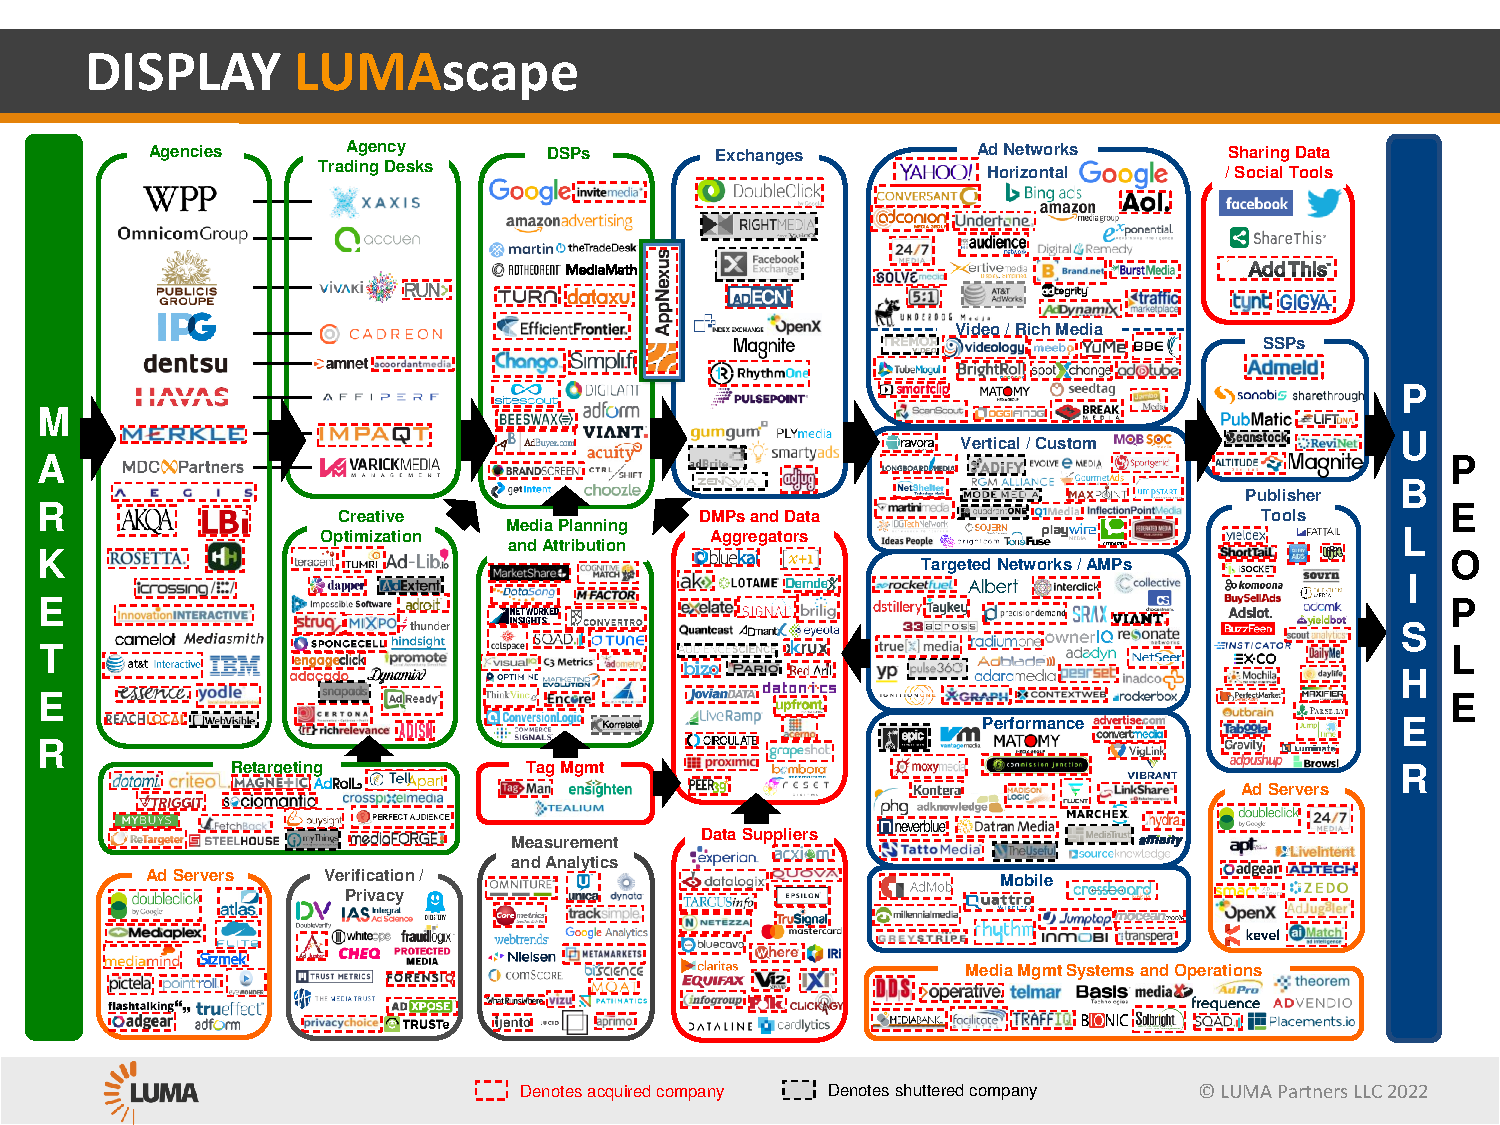
\includegraphics[clip, trim=0cm 0.2cm 0cm 0.2cm, width=0.7\textwidth]{Images/Display_LUMAscape.pdf}  
     \caption{Figure {\color{franklinblue} 8}: Display LUMAscape}
    \label{fig:displayluma}
\end{figure}
\end{frame}

\begin{frame}[t]{Video LUMAscape}
\begin{figure}[htbp]
    \centering
    \captionsetup{justification=centering}
   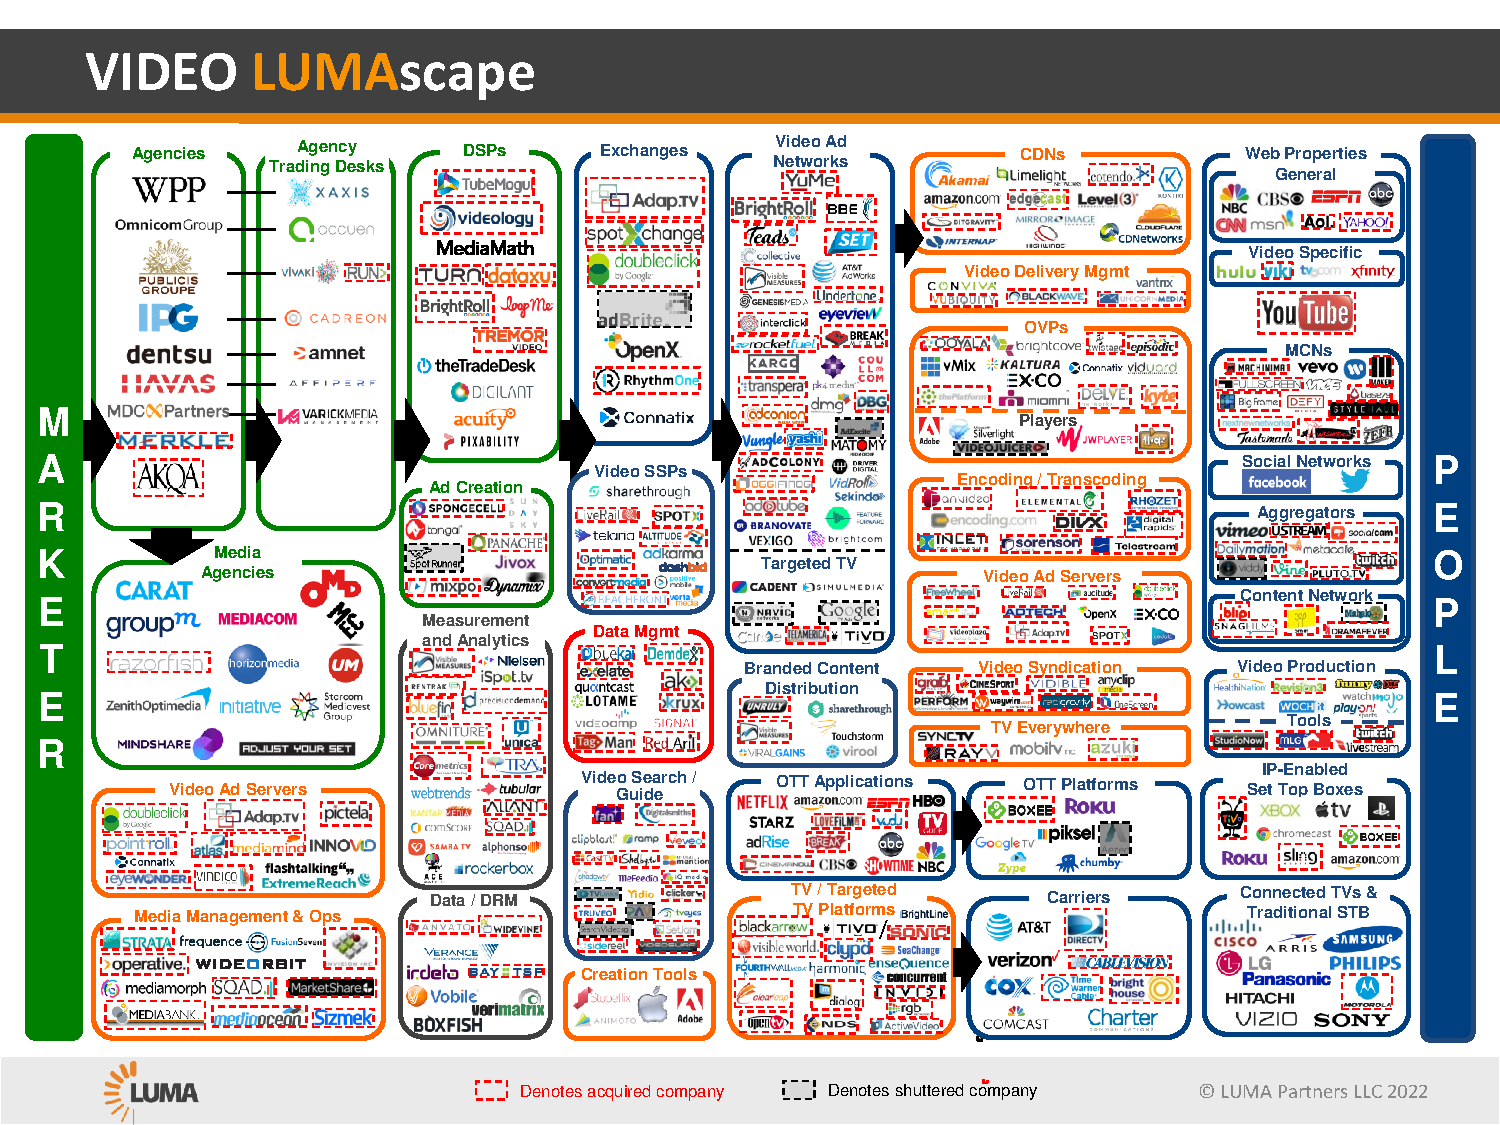
\includegraphics[clip, trim=0cm 0.2cm 0cm 0.2cm, width=0.9\textwidth]{Images/Video_LUMAscape.pdf}  
     \caption{Figure {\color{franklinblue} 9}: Video LUMAscape}
    \label{fig:videoluma}
\end{figure}
\end{frame}

\begin{frame}[t]{Social LUMAscape}
\begin{figure}[htbp]
    \centering
    \captionsetup{justification=centering}
   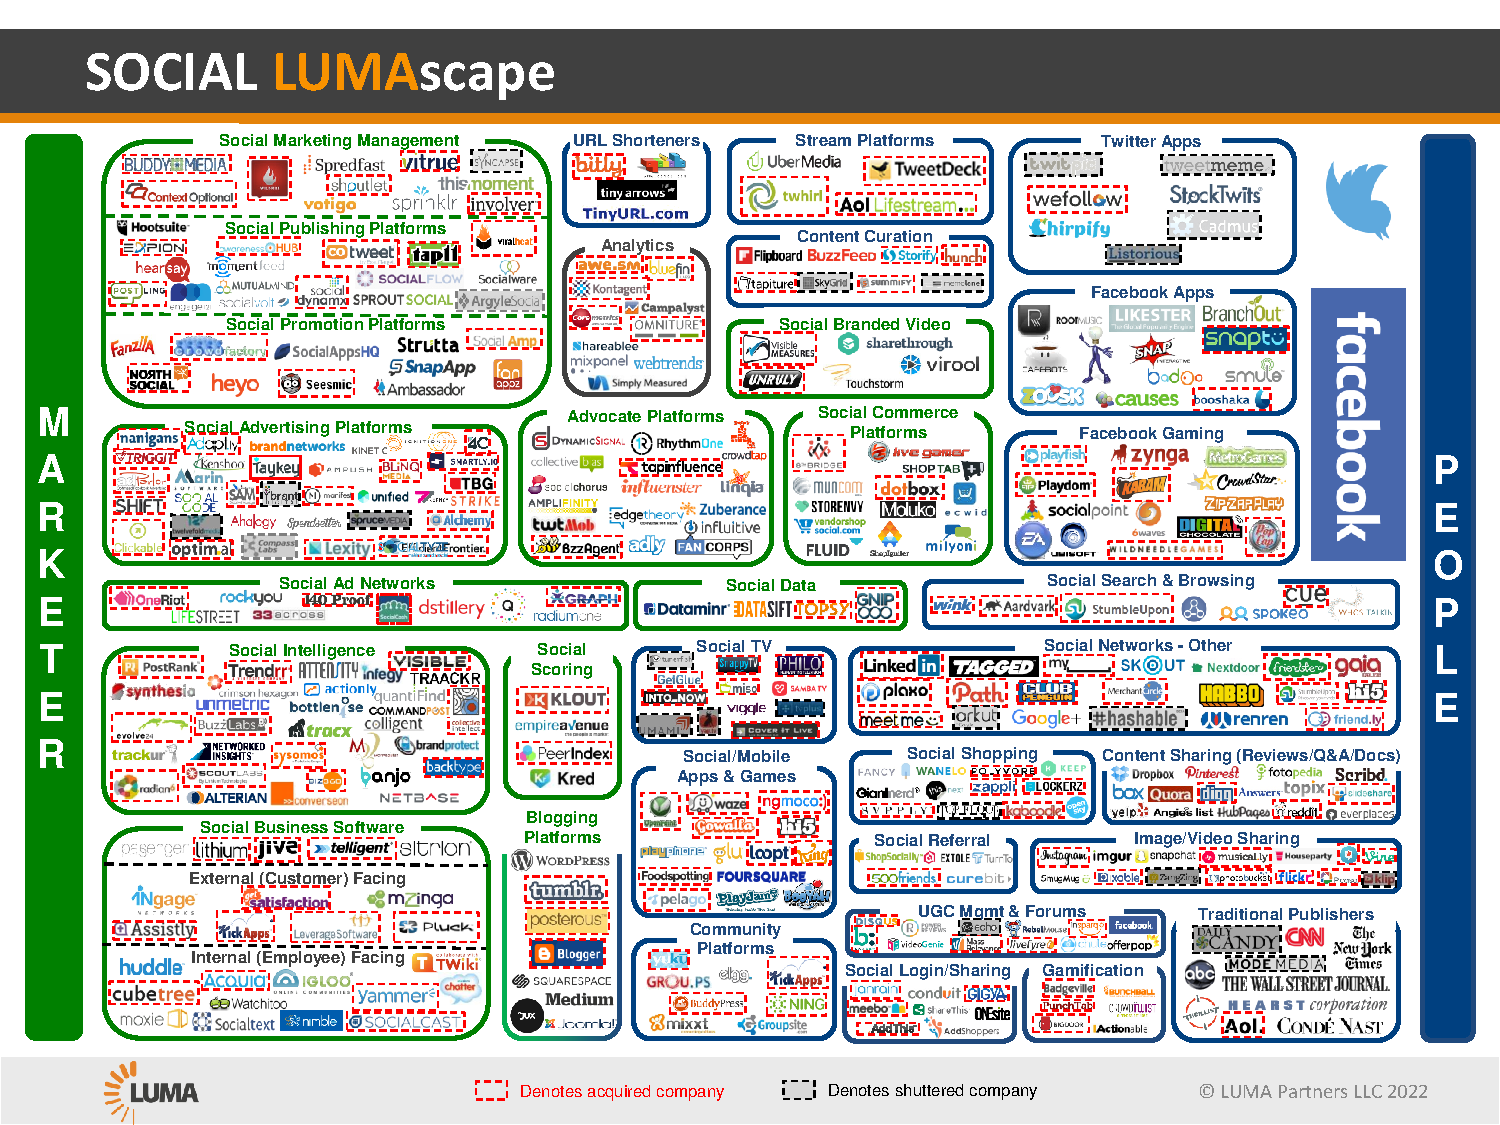
\includegraphics[clip, trim=0cm 0.2cm 0cm 0.2cm, width=0.9\textwidth]{Images/Social_LUMAscape.pdf}  
     \caption{Figure {\color{franklinblue} 10}: Social LUMAscape}
    \label{fig:socialluma}
\end{figure}
\end{frame}

\begin{frame}[t]{Mobile LUMAscape}
\begin{figure}[htbp]
    \centering
    \captionsetup{justification=centering}
    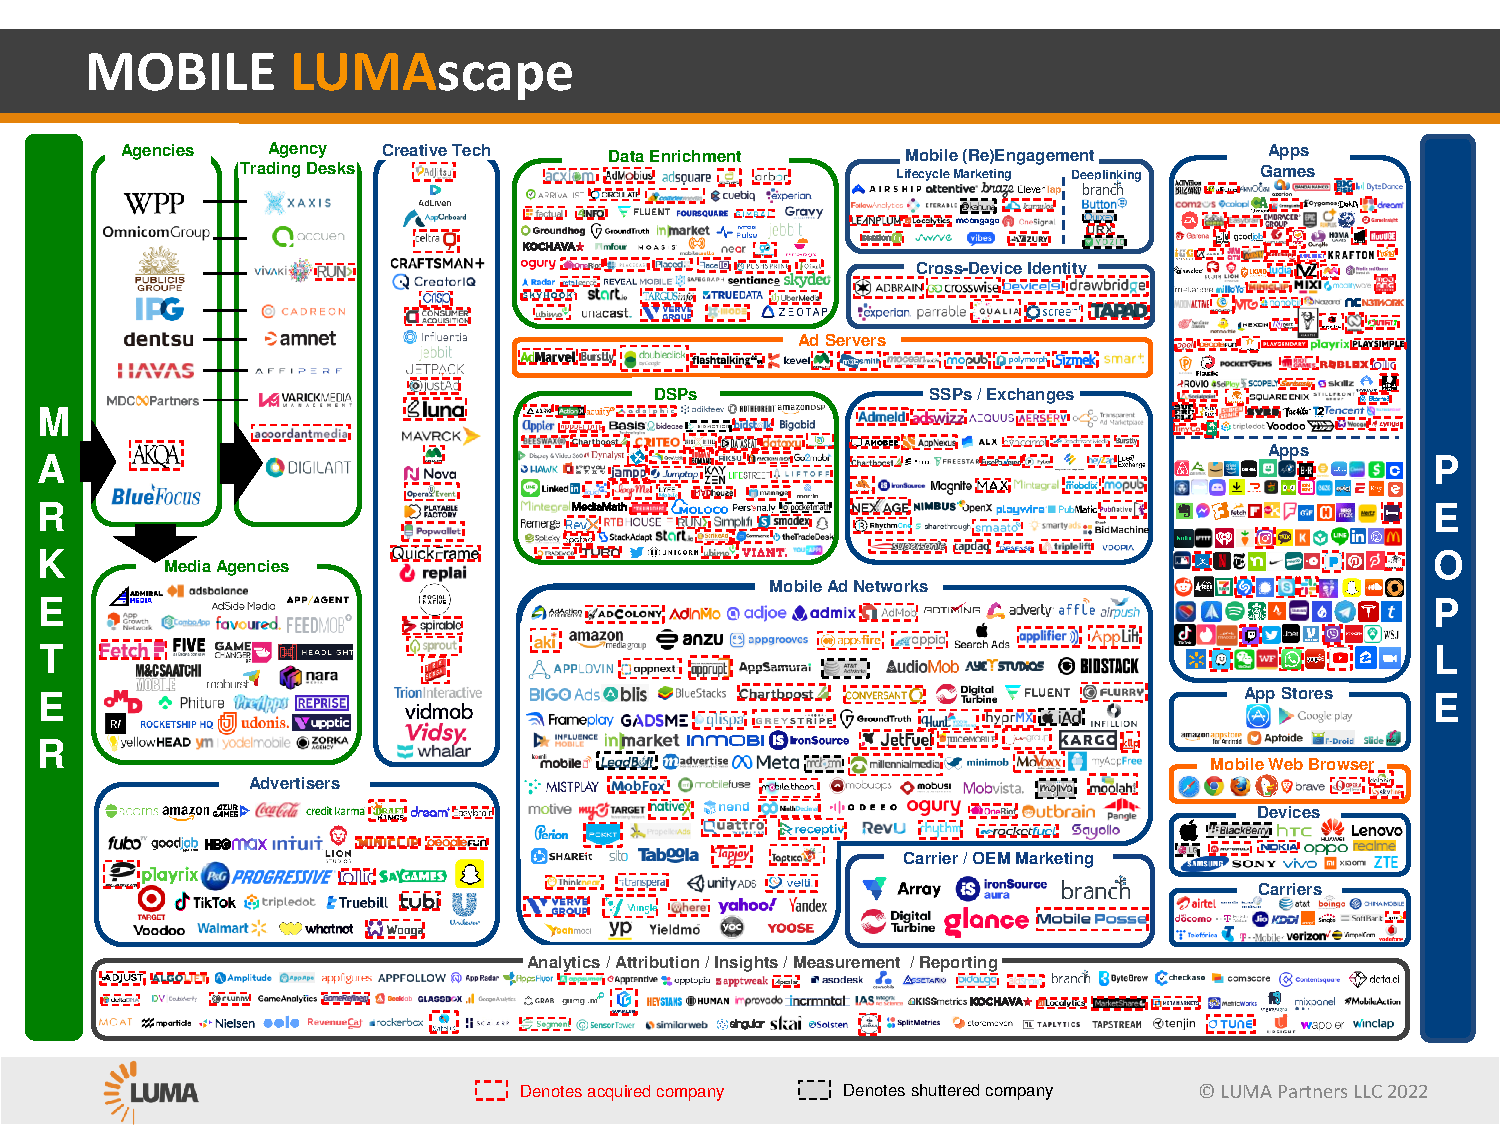
\includegraphics[clip, trim=0cm 0.2cm 0cm 0.2cm, width=0.9\textwidth]{Images/Mobile_LUMAscape.pdf}  
     \caption{Figure {\color{franklinblue} 11}: Mobile LUMAscape}
    \label{fig:mobileluma}
\end{figure}

\end{frame}

\begin{frame}[t]{Convergent TV LUMAscape}
\begin{figure}[htbp]
    \centering
    \captionsetup{justification=centering}
    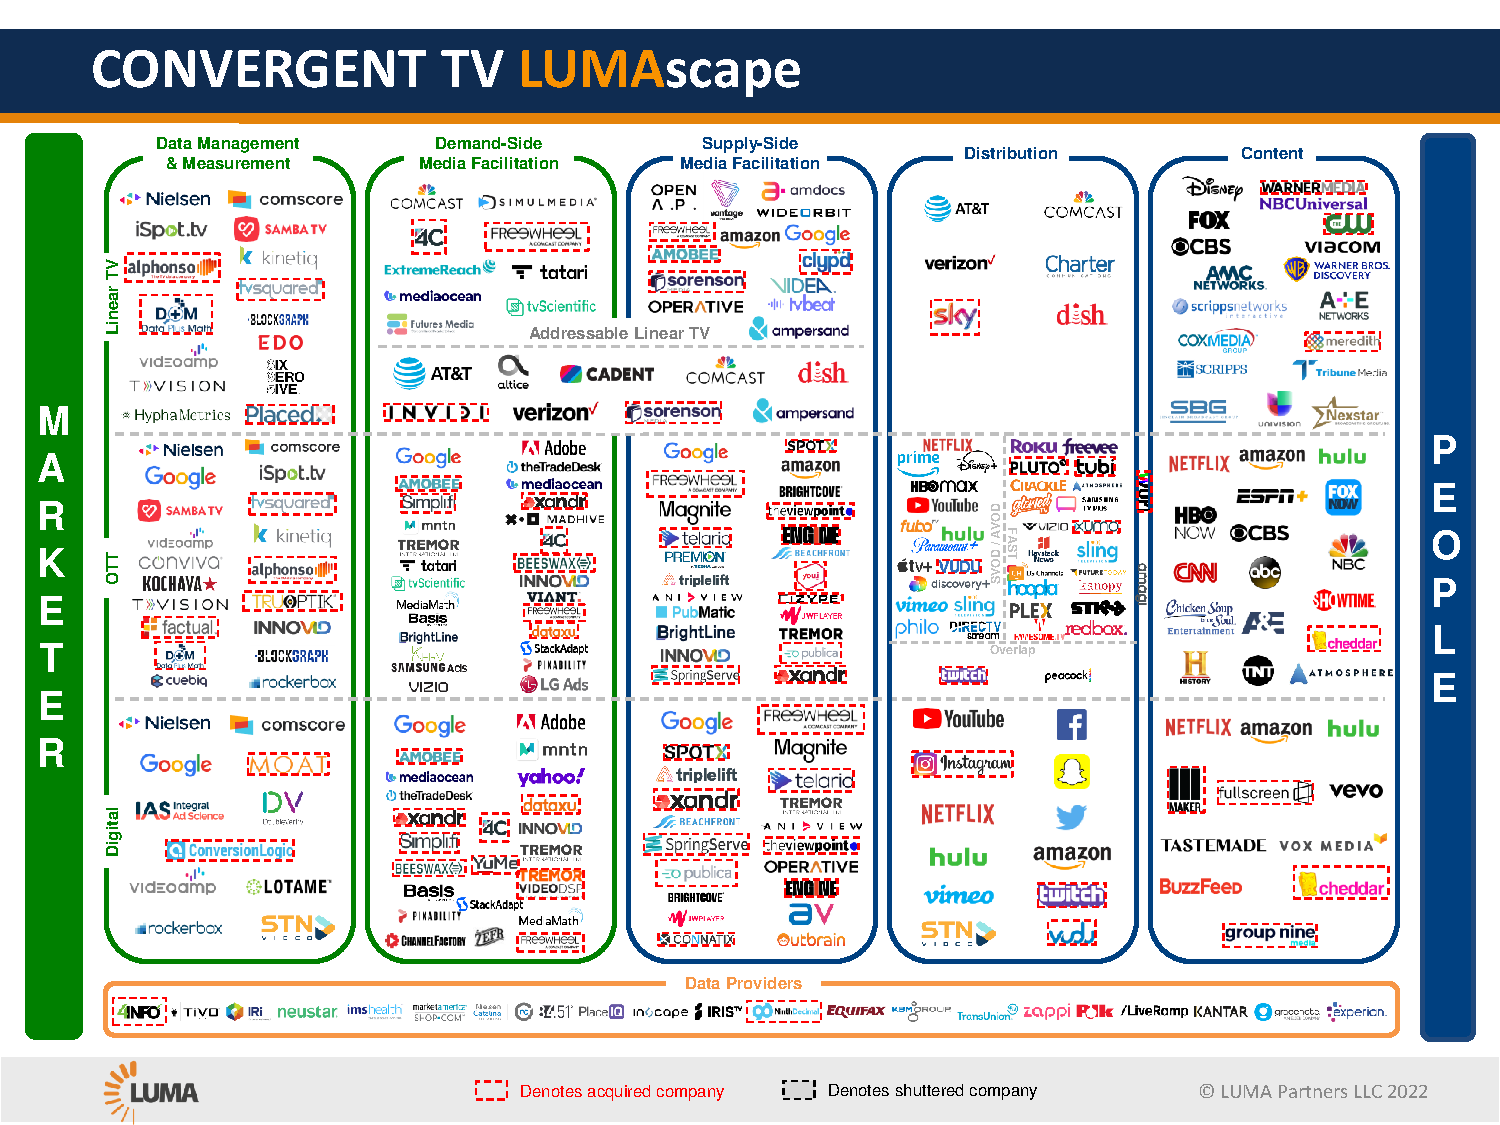
\includegraphics[clip, trim=0cm 0.2cm 0cm 0.2cm, width=0.9\textwidth]{Images/Convergent_TV_LUMAscape.pdf}  
     \caption{Figure {\color{franklinblue} 12}: Convergent TV LUMAscape}
    \label{fig:convergenttvluma}
\end{figure}
\end{frame}

\section{Marketing Measurement and Optimization Solutions}

\begin{frame}[t]{Marketing Mix Models}
The third type of marketing data platform is the \empr{comprehensive marketing measurement and optimization solution}. \\
\vspace{1.5ex}
With both the ability to manage digital content like an inbound marketing tool and the ability to integrate digital and non-digital data like a DMP, comprehensive marketing measurement and optimization solutions also perform predictive analytics and recommend changes to a marketing plan in order to optimize ROI. \\
\vspace{1.5ex}
\empr{Marketing mix models} use data to see what patterns in the present and past can best predict an optimal marketing mix for the future using advanced statistical techniques.  We will review this methodology in detail later during the course.
\end{frame}

\begin{frame}[t]{The Forrester Wave}
The \href{https://www.forrester.com/policies/forrester-wave-methodology/}{Forrester Wave\textsuperscript{TM}} is a guide for buyers considering their purchasing options in a technology marketplace. \\
\vspace{1.5ex}
Results are based on the analysis and opinion of Forrester. \\
\vspace{1.5ex}
Forrester makes publicly available its methodology.  They claim  they apply this methodology consistently across all participating vendors. \\
\vspace{1.5ex}
Sometimes, vendors decide not to participate in the evaluation process. In these instances, Forrester evaluates the vendor according to \href{https://www.forrester.com/policies/wave-vendor-nonparticipation-policy/}{The Forrester New Wave\textsuperscript{TM} Vendor Participation Policy}.\\
\vspace{1.5ex}
\href{https://www.gartner.com/en}{Gartner} is a competitor to Forrester, and has like reports in select verticals. \\
\end{frame}

\begin{frame}[t]{Recent The Forrester Wave MM \& OS Reports}
The following pages present top-line Forrester Wave\textsuperscript{TM} results of their Marketing Measurement and Optimization Solutions (MM \& OS) report.
\begin{itemize}
  \item \href{https://www.forrester.com/report/the-forrester-wave-tm-marketing-measurement-and-optimization-q3-2023/RES178517?ref_search=3539799_1693518171857}{Q3 2023} 
  \item \href{https://www.forrester.com/report/the-forrester-wave-tm-marketing-measurement-and-optimization-solutions-q1-2022/RES176312?ref_search=2100840_1643667194789}{Q1 2022}
  \item \href{https://f.hubspotusercontent00.net/hubfs/1878504/Forrester\%20Wave\%20Report\%202020/The_Forrester_Wave_Marketing\%20Measurement\%20And\%20Optimization\%20Solutions,\%20Q1\%202020.pdf?utm_campaign=Forrester\%20Wave\%20Report\%202020&utm_source=Content\%20Library}{Q1 2020}
  \item \href{https://cdn2.hubspot.net/hubfs/1878504/Forrester\%20Wave\%20Q2\%202018.pdf}{Q2 2018}
\end{itemize}
\vspace{1.5ex}
Figure 1 of each report indicates substantial cross-time vendor performance variation.  Some may believe that such short-term variation is odd. 
\end{frame}

\section{Data Collection Laws}

\begin{frame}[t]{General Data Protection Regulation}
The \href{https://gdpr-info.eu/}{General Data Protection Regulation} 
(GDPR) was the first standardized data collection law. It went into effect on May 25, 2018, in \href{https://european-union.europa.eu/principles-countries-history/country-profiles_en}{European Union} (EU) countries. \\
\vspace{1.5ex}
\begin{itemize}
  \item It protects a natural person's right to the protection of personal data.\footnote{A natural person is a living, breathing human being.}
  \item It stipulates that the free movement of personal data within the EU shall be neither restricted nor prohibited for reasons connected with the protection of natural persons with regard to the processing of personal data.
  \item  For especially severe violations the 
  \href{https://gdpr-info.eu/issues/fines-penalties/\#:~:text=83(4)\%20GDPR\%20sets\%20forth,to\%20that\%20used\%20in\%20Art}{fine framework} 
  can be up to 20 million euros, or in the case of an undertaking, up to 4\% of their total global turnover (i.e., gross revenue) of the preceding fiscal year, whichever is larger.
\end{itemize}
\end{frame}

\begin{frame}[t]{California Consumer Privacy Act}
The \href{https://oag.ca.gov/privacy/ccpa}{California Consumer Privacy Act} of 2018 (CCPA) gives consumers in California more control over the personal information that businesses collect about them. The law secures new privacy rights for California consumers, including:\\
\vspace{1.5ex}
\begin{itemize}
  \item The right to know about the personal information a business collects about them and how it is used and shared.
  \item The right to delete personal information collected from them (with some exceptions).
  \item The right to opt-out of the sale of their personal information.
  \item The right of non-discrimination for exercising their CCPA rights.
\end{itemize}
\end{frame}

\begin{frame}[t]{Business Ramifications}
 As mentioned in the Appendix of Module 1, companies like Google and Apple responded respectively by phasing out the use of \href{https://blog.google/products/chrome/update-testing-privacy-sandbox-web/}{third-party cookies in Chrome browsers} and \href{https://support.apple.com/en-us/HT212025}{prompting iPhone users} to choose whether they would like to be tracked by each of their apps, respectively. %\footnote{A \empr{cookie} is a string of text sent from a web server to a user's browser that the browser is expected to send back to the web server in subsequent interactions. A \empr{third-party cookie} is a cookie placed on a website by some entity other than the owner of the website, and collects user data for the third party.  For example, DMP cookies are third-party. The Interactive Advertising Bureau (IAB) has an excellent \href{https://www.iab.com/insights/glossary-of-terminology/\#index-3}{glossary} of media terms.}
 \\
 \vspace{1.5ex} 
 These decisions, and forthcoming decisions, affect marketing analytics.  Beyond the alternatives that were mentioned in the Appendix of Module 1, which are now used or could be used, the following have been used or may be used.
\begin{enumerate}
  \item A \empr{walled garden} is an environment that controls the user's access to network-based content and services.\footnote{For example, Google has Account IDs that can be linked to first-party user IDs.  Google shares some of its first-party data, usually via a data privacy mechanism, with the firm who has linked its IDs with the Google Account IDs.}
\end{enumerate}
\end{frame}

\begin{frame}[t]{Cooked Data and Topics}
\begin{enumerate}
\setcounter{enumi}{1} 
  \item  \empr{Cooked data} are  raw data that has been processed, which may include data that is inferred or imputed.\footnote{For example, if a data set has geographical information about a person such as their zip code, it is possible to infer additional data like income, age or purchase habits, information that is no longer as pervasive due to the consumer protection laws.} 
  \item Google has put forward \href{https://blog.google/products/chrome/get-know-new-topics-api-privacy-sandbox/}{Topics}, a new Privacy Sandbox proposal for interest-based advertising. 
\begin{itemize}
  \item Google has a list of 300 topics (for now) that they use to categorize the websites people visit. When a person visits a new website, Google will categorize it into whatever topic it fits best.  
  \item Topics will only show advertising partners three of your interests. It pulls one interest from each week to share with advertisers.
\end{itemize}
\end{enumerate}
\end{frame}

\begin{frame}[t]{Economic Consequences of GDPR}
\cite{goldberg2024} study the economic consequences of GDPR for a large and diverse collection of online firms.  They examine the effect of GDPR on site traffic, a measure of site health and its capacity to generate advertising revenue, and site revenue arising from e-commerce sales.  \\
\vspace{1.5ex}
Using Adobe Analytics website performance data of 1,084 firms, they show that relative to the prior year recorded page views decrease by 11.7\% and e-commerce revenue decreased 13.3\% from EU users after GDPR implementaion. \\
\vspace{1.5ex}
\begin{itemize}
\item However, the data alone do not distinguish between the real and recording effects of the GDPR. 
\item They propose a model to separate GDPR's real effect on the volume of site visits and the GDPR's consent effect on the recording of site visit outcomes. 
\end{itemize}
\end{frame}

\begin{frame}[t]{Economic Consequences of GDPR Continued}
  \begin{itemize}
    \item [] 
    \begin{itemize}
      \item Under the GDPR recorded economic outcomes may fall because some individuals \underline{do not consent} to data sharing. Indeed, changes to when and what data are recorded is a primary goal of the GDPR. 
      \item At the same time, a decline in recorded outcomes could reflect a \underline{decline in real economic outcomes}, for instance because the regulation restricts personalized marketing.
      \item  Privacy regulation thus creates an inference problem: data protection can both impact economic outcomes and obscure the observation of economic outcomes. Thus policymakers need to distinguish between the real and recording effects of privacy regulation in order to evaluate it.
    \end{itemize}
  \end{itemize}
\end{frame}

\begin{frame}[t]{Economic Consequences of GDPR Continued}
\begin{itemize}
\item They conclude that consent accounts for at least 4.7\% of the recorded page view estimate. 
\item They also provide conservative estimates for the contribution of GDPR's real effect on personalized marketing. The marketing effect alone represents 7.0\% of the recorded page view estimate and 4.6\% of the recorded revenue estimate.
\item Despite concerns of consent fatigue, a substantial minority of EU users make the effort to register their nonconsent preferences. The authors provide evidence that smaller firms obtain lower consent rates, which suggests GDPR may have consequences for competition.
\end{itemize}
\end{frame}

\section{Appendix}

\begin{frame}[t]{Airflow Workflow}
Airflow is a platform that lets one build and run workflows. A workflow is represented as a \href{https://airflow.apache.org/docs/apache-airflow/stable/concepts/dags.html}{directed acyclic graph} (DAG), and contains individual pieces of work called \href{https://airflow.apache.org/docs/apache-airflow/stable/concepts/tasks.html}{tasks}, arranged with dependencies and data flows taken into account. \\
\vspace{1.5ex}
A DAG specifies the dependencies between asks, and the order in which to execute them and run retries; the tasks themselves describe what to do, be it fetching data, running analysis, triggering other systems, or more. \\
\vspace{1.5ex}
\begin{figure}[htbp]
  \captionsetup{justification=centering}
  \includegraphics[height=2cm, trim=0.0cm 0.0cm 0.0cm 0.0cm width=2cm]{Images/AirFlow_DAG_Example.png}
  \caption{Figure {\color{franklinblue} 13}: An Illustrative Airflow DAG}
\end{figure}
\end{frame}

\begin{frame}[t]{Introduction to the Airflow Architecture}
%https://airflow.apache.org/docs/apache-airflow/stable/concepts/overview.html
An Airflow installation generally consists of the following components: \\
\vspace{0.0ex}
\small
\begin{itemize}
  \item A \href{https://airflow.apache.org/docs/apache-airflow/stable/concepts/scheduler.html}{scheduler}, which handles both triggering scheduled workflows, and submitting tasks to the executor to run. 
  \item An \href{https://airflow.apache.org/docs/apache-airflow/stable/executor/index.html}{executor}, which handles running tasks. In the default Airflow installation, this runs everything inside the scheduler, but most production-suitable executors actually push task execution out to workers.
  \item A \href{https://developer.mozilla.org/en-US/docs/Learn/Common_questions/What_is_a_web_server}{web server}, which presents a handy user interface to inspect, trigger and debug the behavior of DAGs and tasks.
  \item A folder of DAG files, read by the scheduler and executor, and any workers the executor has.
  \item A \href{https://docs.astronomer.io/learn/airflow-database}{metadata database}, used by the scheduler, executor and web server to store the state of the process.
\end{itemize}
\end{frame}

\begin{frame}[t]{Airflow Architecture Visual}
\begin{figure}[htbp]
  \captionsetup{justification=centering}
  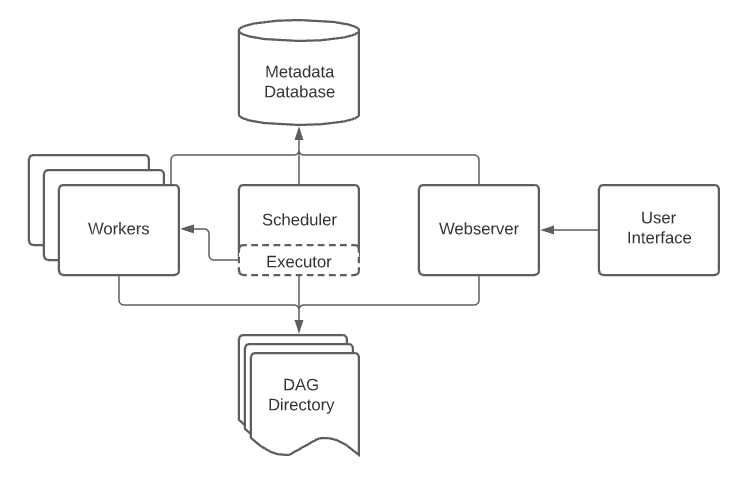
\includegraphics[height=7cm, trim=0.0cm 0.0cm 0.0cm 0.0cm width=7cm]{Images/AirFlow_Orchestration.png}
  \caption{Figure {\color{franklinblue} 14}: Airflow Architecture}
\end{figure}
\end{frame}

\section{References}

\begin{frame}[t,allowframebreaks]
%https://latex-beamer.com/faq/long-bibliographies-beamer/
%https://github.com/jgm/pandoc/issues/2442
\widowpenalties 1 10000
\small
\bibliography{../../Bibliography/list2}
\bibliographystyle{apalike}
\end{frame}

\end{document}